\documentclass[%
candidate,   % тип документа
subf,        % использовать пакет subcaption для вложенной нумерации рисунков
href,        % использовать пакет hyperref для создания гиперссылок
colorlinks,  % цветные гиперссылки
%times,      % шрифт Times как основной
%fixint,     % включить прямые знаки интегралов
%classified, % гриф секретности
%facsimile,  % отображать факсимиле диссертанта
]{disser}

\usepackage[
  a4paper, mag=1000,
  left=2.5cm, right=1cm, top=2cm, bottom=2cm, headsep=0.7cm, footskip=1cm
]{geometry}
\usepackage[T2A]{fontenc}
\usepackage[utf8]{inputenc}
\usepackage[english,russian]{babel}
\usepackage{csquotes}
\ifpdf\usepackage{epstopdf}\fi
\usepackage{amsmath, amsthm, amssymb}
\usepackage{lastpage}
\usepackage{multirow}
\usepackage{setspace}
\usepackage{float}
\linespread{1.6} %1.3 для полуторного
%\usepackage{multibib}
\usepackage{longtable}

\usepackage[style=gost-numeric,
  backend=biber,
  language=auto,
  hyperref=auto,
  autolang=other,
  sorting=nyt,
  defernumbers=true
]{biblatex}

\addbibresource{thesis.bib}
%\bibliography{thesis}

% Номера страниц снизу и по центру
\pagestyle{footcenter}
\chapterpagestyle{footcenter}

% Точка с запятой в качестве разделителя между номерами цитирований
%\setcitestyle{semicolon}

% Ссылки на работы соискателя включаются в общий список литературы
%\let\citemy=\cite

%\newcites{mybib}{Публикации автора по теме диссертации}

% Использовать полужирное начертание для векторов
\let\vec=\mathbf

\newtheorem{theorem}{Теорема}[chapter] 
\newtheorem{cor}{Следствие} 
\newtheorem{lemma}{Лемма}[chapter]
\newtheorem{fact}{Утверждение}[chapter]
\newtheorem{remark}{Замечание}[chapter]

% Путь к файлам с иллюстрациями
\graphicspath{{fig/}}

\begin{document}

% Переопределение стандартных заголовков
%\def\contentsname{Содержание}
%\def\conclusionname{Выводы}
%\def\bibname{Литература}

% Включение файла с общим текстом диссертации и автореферата
% (текст титульного листа и характеристика работы).
% Общие поля титульного листа диссертации и автореферата
\institution{Название организации}

\topic{Тема диссертации}

\author{Скурыдина Алия Фиргатовна}

\specnum{01.01.07}
\spec{Вычислительная математика}
%\specsndnum{01.04.07}
%\specsnd{Физика конденсированного состояния}

\sa{Акимова Елена Николаевна}
\sastatus{д.~ф.-м.~н., доц.}
%\sasnd{ФИО второго руководителя}
%\sasndstatus{к.~ф.-м.~н., проф.}

%\scon{ФИО консультанта}
%\sconstatus{д.~ф.-м.~н., проф.}
%\sconsnd{ФИО второго консультанта}
%\sconsndstatus{д.~ф.-м.~н., проф.}

\city{Екатеринбург}
\date{\number\year}

% Общие разделы автореферата и диссертации
\mkcommonsect{actuality}{Актуальность темы исследования.}{%
Построение итеративно регуляризованных алгоритмов востребовано для решения широкого круга прикладных некорректно поставленных задач. Так, решение структурных обратных задач гравиметрии и магнитометрии сводится к решению нелинейных интегральных уравнений Урысона первого рода. После дискретизации операторное уравнение сводится к системе нелинейных уравнений с большим числом неизвестных, поэтому есть необходимость в параллелизации алгоритмов для многопроцессорных и многоядерных вычислительных систем с целью уменьшения времени счета. 
}

\mkcommonsect{development}{Степень разработанности темы исследования.}{
Ж. Адамар в 1902 г.~\cite{Hadamar1902} впервые определил условия корректности задачи математической физики. Задачи, не отвечающие этим условиям, то есть некорректные,  Ж. Адамар считал лишенными физического смысла. В течение многих лет обратные задачи решались методом подбора, например, в геофизике, сравнивая вычисленное физическое поле модели с наблюденным. Однако со временем, это мнение претерпело изменения.

Первой работой по теории некорректных задач считается известная работа академика А.Н. Тихонова 1943 г.~\cite{Tikh1943}, в которой он доказал устойчивость некоторых обратных задач при условии принадлежности решения компактному множеству. Также в этой работе он решил одну из актуальных обратных задач разведочной геофизики. В дальнейшем теория некорректных задач оформилась в самостоятельный раздел современной математики. В конце 50-х годов и начале 60-х годов появились работы, посвященные решению некоторых некорректных задач с помощью идей регуляризации, выдающихся отечественных ученых: А.Н. Тихонова, М.М. Лаврентьева, В.К. Иванова. Их исследования в этой области положили начало трем научным школам:  Московской, Сибирской и Уральской.
Началось исследование устойчивых методов решения некорректно-поставленных задач, представляющих собой одно из наиболее актуальных проблем современной математической науки.

В большом цикле работ, выполненных начиная с 1963 года, А.Н. Тихонов сформулировал принцип устойчивого решения некорректно-поставленных задач, ввел понятие регуляризирующего оператора и предложил ряд эффективных методов построения таких операторов, легко реализуемых на ЭВМ ~\cite{Tikh1963_1, Tikh1963_2, TikhGlas1965, TikhArs1986}. Метод, получивший название "метод регуляризации А.Н. Тихонова"\, был применен для решения большого количества как фундаментальных математических, так и актуальных прикладных задач. В частности, тихоновским методом регуляризации были решены задача об отыскании решения интегрального и операторного уравнения первого рода, обратные задачи теории потенциала и теплопроводности. 

Наряду с Тихоновым, М.М. Лаврентьев изучал методы регуляризации. Ему принадлежит идея замены исходного уравнения близким ему, в некотором смысле, уравнением, для которого задача нахождения решения устойчива к малым изменениям правой части и разрешима для любой правой части ~\cite{Lavr1962}. Были доказаны теоремы сходимости регуляризованного решения к точному ~\cite{Lavr1956}. Основополагающие  результаты  для  интегральных  уравнений  Фредгольма  первого  рода  получены  в  ~\cite{Lavr1959, Lavr1963, LavrVas1966, LavrRomShi1980},  где  для  решения  линейных  интегральных  уравнений  Фредгольма  первого  рода  построены  регуляризирующие  операторы  по  М.М. Лаврентьеву. 

В работах Иванова, выполненных в 1960--1970-е гг., было введено понятие квазирешения ~\cite{Iv1962_2, Iv1963}, были заложены также основы двусторонних оценок регуляризующих алгоритмов ~\cite{Iv1966}, установлены связи между вариационными методами регуляризации, развит единый подход к трактовке линейных некорректных задач в топологических пространствах ~\cite{Iv1967}. 

Однако не все некорректные задачи возможно регуляризовать. Так, российский математик Л.Д. Менихес ~\cite{Menih1978} привел пример интегрального оператора с непрерывным замкнутым ядром, действующего из пространства \( C[0,1] \) в \( L_2[0,1] \), обратная задача для которого нерегуляризуема. Проблемам регуляризуемости также посвящены работы Ю.И. Петунина и А.Н. Пличко ~\cite{PetPlich1980}.

Для построения регуляризующих алгоритмов для решения прикладных задач требуется использовать дополнительную информацию о свойствах искомого решения, заданную в виде равенств и неравенств, характеристик решения, например, свойствами гладкости, естественно вытекающих из физической сущности задачи. Получило развитие построение регуляризующих алгоритмов вариационными методами. А.Б. Бакушинский, Б.Т. Поляк сформулировали общие принципы построения регуляризующих алгоритмов в банаховых пространствах \cite{BakPol1974}. Метод обобщенной невязки был предложен А.В. Гончарским, А.С. Леоновым, А.Г. Яголой \cite{GonLeoYag1973}.  Монография А.Б. Бакушинского, А.В. Гончарского \cite{BakGon1989} посвящена итеративной регуляризации вариационных неравенств с монотонными операторами, которые единообразно описывают многие постановки задач с априорной информацией. В работе \cite{Bak1992} А.Б. Бакушинский предложил модификацию метода Гаусса -- Ньютона в духе итеративной регуляризации и исследовал его на сходимость. Метод
Гаусса -- Ньютона был также исследован в работах B. Blaschke, A. Neubauer, O. Scherzer, B. Kaltenbacher, A.G.Ramm \cite{BlaNeuSch1997,KalNeuRam2002}.

Методам решения операторных уравнений первого рода посвящены работы В.П. Тананы~\cite{Tan1977, Tan1997} и монография \cite{Tan1981}. Им был введен метод $L$-регуляризации, представляющий собой разновидность метода Тихонова, расширивший класс регуляризуемых задач \cite{Tan2003_1,Tan2003_2}.

Регуляризующие алгоритмы в пространствах функций ограниченной вариации были впервые предложены М.Г. Дмитриевым, В.С. Полещуком \cite{DmiPol1972}, И.Ф. Дорофеевым \cite{Dor1979}. Далее в работах А.В. Гончарского и В.В. Степанова \cite{GonSte1979} А.Л. Агеева \cite{Ag1980} была доказана равномерная сходимость приближенных решений. Подход, изложенный в \cite{TikhGonSteYag1990} основан на идее двухэтапного алгоритма: построении приближенного решения  исходного операторного уравнения из условия минимизации регуляризованной невязки на априорном множестве, где привлекается информация о неотрицательности, монотонности и выпуклости решения: $$min\{\| A(u)-f_\delta\| ^2 + \alpha \Omega(u): u\in\Omega, \|f-f_\delta\|\le\delta \},$$ 
где $A$ --- оператор задачи, $f$ --- правая часть без шума, $f_\delta$ --- возмущенная правая часть, $\delta$ --- уровень шума, $\alpha$ --- параметр регуляризации. 

На втором этапе для решения корректно поставленной экстремальной задачи применяются методы градиентного типа, линеаризованные методы, или алгоритмы, специально ориентированные на определенный класс априорных ограничений.

Для решения систем нелинейных уравнений предложены методы в работах Л.В. Канторовича \cite{Kan1947}, Б.Т. Поляка \cite{Pol1969}, J. M. Ortega и W. C. Rheinboldt \cite{OrtRhe1970}, A. Neubauer, O. Scherzer \cite{NeuSch1995, Sch1995}, M.J.D. Powell \cite{Pow1970}, J.E.Dennis, R.B. Schnabel, P.D. Frank \cite{DenSchn1996}, C.T. Kelley \cite{Kel1995}, R.B. Schnabel и P.D. Frank \cite{SchnFra1983} для решения систем уравнений с сингулярной или плохо обусловленной матрицей Якоби, J.C. Gilbert, J. Nocedal, S.J. Wright \cite{GilNoc1991, NocWri2006}. Термин $\alpha$-процессы, характеризующий класс нелинейных итерационных методов (где оператор шага нелинеен) для решения линейного уравнения с ограниченным самосопряженным положительно полуопределенным оператором был введен в монографии М.А. Красносельского, Г.М. Вайникко, П.П. Забрейко \cite{KraVayZab1969}. Сходимость и устойчивость методов наискорейшего спуска и минимальной ошибки исследовалась авторами A. Neubauer, O. Scherzer в \cite{NeuSch1995}.

L. Landweber в статье \cite{Lan1951} 1951 г. предложил метод для решения линейных интегральных уравнений Фредгольма I рода. В дальнейшем авторы M. Hanke, A. Neubauer и O. Scherzer \cite{HanNeuSch1995,Neu2000,NeuSch1995} применили метод Ландвебера для решения нелинейных нерегулярных уравнений, доказали теоремы о сходимости и исследовали скорость сходимости метода. Градиентные методы с применением метода Ландвебера исследовались М.Ю. Кокуриным в работах \cite{Kok2010_1,Kok2010_2}.

В работах \cite{Han1997,Han2010} M. Hanke предложил новую схему метода Левенберга -- Марквардта для решения некорректных задач на примере задачи фильтрации.

В.В. Васиным предложен подход к решению задач с априорной информацией в работах ~\cite{Vas1982, Vas1988} и в монографиях ~\cite{VasAge1993, VasEre2005}, основанный на применении фейеровских отображений для учета априорных ограничений в форме выпуклых неравенств. Термин <<фейеровское отображение>> введен Ереминым в работах ~\cite{Ere1965, Ere1966, Ere1968} в честь венгерского математика Фейера. Отображения, обладающие свойством фейеровости, позволяют строить итерационные процессы с учетом априорных ограничений достаточно общего вида и, в отличие от метрической проекции, допускают эффективную реализацию. На основе $\alpha$-процессов были предложены регуляризованные методы решения линейных операторных уравнений Фредгольма $I$ рода, возникающих, например, при решении линейных обратных задач гравиметрии. Также Васин доказал сильную сходимость метода Левенберга -- Марквардта и его модифицированного варианта для решения регуляризованного по Тихонову нелинейного уравнения. Были приведены численные эксперименты для нелинейной обратной задачи гравиметрии в работах В.В. Васина и Г.Я. Пересторониной~\cite{VasPer2011}, В.В. Васина ~\cite{Vas2012}. Они показали, что основной процесс Левенберга -- Марквардта существенно превосходит по точности модифицированный вариант и не требует жестких условий на начальное приближение, но обладает большей вычислительной сложностью, и, следовательно, требует больших затрат машинного времени.

При исследовании методов решения некорректных задач важное место занимает оценка погрешности регуляризованного решения по отношению к точному решению. Для уравнения с монотонным оператором исследовался метод Лаврентьева U. Tautenhahn \cite{Tau2002,Tau2004}, стратегия выбора параметра регуляризации по Тихонову исследовался авторами Q. Jin Zong-Yi Hou, O. Scherzer, H. W. Engl и K. Kunisch \cite{JinZon1997,JinZon1999,SchEngKun1993}. В.П. Тананой была доказана сходимость решения $L$-регуляризованной вариационной задачи к решению исходного операторного уравнения $I$ рода, продемонстрировав на примере двумерной обратной задачи гравиметрии \cite{Tan2003_2}.
}

\mkcommonsect{objective}{Цели и задачи диссертационной работы:}{%
построить новые методы решения нелинейных операторных уравнений первого рода в гильбертовом пространстве, исследовать их сходимость. Предложить методы решения обратной задачи гравиметрии, использующие особенности физической модели.
%
%Для достижения поставленных целей были решены следующие задачи:
%\begin{itemize}
%	\item для нелинейного уравнения с монотонным оператором доказаны теоремы сходимости для регуляризованного метода Гаусса -- Ньютона, доказана сильная фейеровость итерационных процессов;
%	\item построены регуляризованные методы градиентного типа, названные нелинейными аналогами $\alpha$-процессов, для нелинейного уравнения с монотонным оператором доказаны теоремы сходимости для них, доказана сильная фейеровость итерационных процессов;
%	\item для задачи с немонотонным оператором с производной, имеющей неотрицательный спектр, доказаны теоремы сходимости методов Ньютона, нелинейных $\alpha$-процессов и их модифицированных вариантов;
%	\item предложена вычислительная оптимизация метода Ньютона и его модифицированного варианта при решении задач с матрицей производной, близкой к ленточной;
%	\item lля решения систем нелинейных интегральных уравнений  с ядром оператора структурной обратной задачи гравиметрии в двуслойной среде предложен покомпонентный метод, основанный на методе Ньютона;
%	\item для решения систем нелинейных уравнений  структурных обратных задач гравиметрии в многослойной среде предложен подход на основе метода Левенберга -- Марквардта --- покомпонентный метод типа Левенберга --- Марквардта;
%	\item проведены численные эксперименты, интерпретированы результаты.
%\end{itemize}
}

\mkcommonsect{novelty}{Научная новизна.}{%
Результаты, полученные в диссертационной работе, являются новыми и состоят в следующем:

	в рамках двухэтапного метода построения регуляризующего алгоритма обоснованы сходимость метод Ньютона и нелинейные аналоги альфа-процессов: метод минимальной ошибки (ММО), метод наискорейшего спуска (МНС) и метод минимальных невязок (ММН). Также установлена сходимость модифицированных вариантов методов ММО, МНС, ММН, когда производная оператора вычисляется в начальной точке итераций. Рассмотрены два случая: оператор задачи является монотонным, либо оператор является конечномерным и его производная имеет неотрицательный спектр.
	
	Для решения систем нелинейных интегральных уравнений  с ядром оператора структурной обратной задачи гравиметрии в двуслойной среде предложен покомпонентный метод, основанный на методе Ньютона. 
	Предложена вычислительная оптимизация метода Ньютона и его модифицированного варианта в виде перехода от плотно заполненной матрицы производной оператора к ленточной в силу особенности строения ядер интегральных операторов задач грави- магнитометрии.
	Для решения систем нелинейных уравнений  структурных обратных задач гравиметрии в многослойной среде предложен подход на основе метода Левенберга-Марквардта – покомпонентный метод типа Левенберга-Марквардта.

}

\mkcommonsect{value}{Теоретическая и практическая значимость.}{%
Результаты, изложенные в диссертации, могут быть использованы для решения нелинейных операторных уравнений, в частности, задач гравиметрии и магнитометрии.
}

\mkcommonsect{methods}{Методология и методы исследования.}{%
Текст о методах исследования.
}

\mkcommonsect{results}{Положения, выносимые на защиту:}{%
1. Сформулированы и доказаны теоремы, устанавливающие сильную фейеровость оператора шага итераций методов:
	\begin{itemize}
		\item 	метод Ньютона;
		\item	метод минимальной ошибки и его модифицированный вариант;
		\item	метод наискорейшего спуска и его модифицированный вариант;
		\item	метод минимальных невязок и его модифицированный вариант.
	\end{itemize}
	
	Доказана сильная фейеровость оператора шага итераций данных методов в случае монотонного оператора задачи и в случае конечномерного оператора с производной, имеющей неотрицательный спектр. Доказывается линейная скорость сходимости итерационных процессов.
	
	2. Предложена вычислительная оптимизация метода Ньютона, которая в задачах гравиметрии и магнитометрии обеспечивает более высокую точность численного решения, а также уменьшает время счета программ.
	
	3. Предложены покомпонентные методы:
		\begin{itemize}
			\item покомпонентный основанный на методе Ньютона для решения нелинейного интегрального уравнения в задаче гравиметрии в двухслойной среде;
			\item покомпонентный метод типа Левенберга-Марквардта для решения систем нелинейных уравнений  структурных обратных задач гравиметрии в многослойной среде.
		\end{itemize} Данные методы обладает меньшей вычислительной сложностью в отличие от классических методов Ньютона и Левенберга-Марквардта.
		
Вычислительные эксперименты показывают, что предложенные метод позволяют существенно уменьшить вычислительную сложность задачи и являются экономичными по потреблению памяти ЭВМ.
		
		4. Проведены численные эксперименты для модельных и квазиреальных геофизических данных, разработан комплекс параллельных программ для многоядерных и графических процессоров с использованием технологий OpenMP, CUDA. 
}

\mkcommonsect{approbation}{Степень достоверности и апробация результатов.}{%
Основные результаты по материалам диссертационной работы докладывались на конференциях:

1. XIV и XV Уральская молодежная научная школа по геофизике (Пермь, 2013 г., Екатеринбург 2014 г.);

2. Международная коференция "Параллельные вычислительные технологии" (Ростов-на-Дону, 2014 г., Екатеринбург, 2015 г., Казань, 2017 г.);

3. Международная конференция «Геоинформатика: теоретические и прикладные аспекты» (Киев 2014, 2015, 2016 г.)

4. Международная конференция "Актуальные проблемы вычислительной и прикладной математики" (Новосибирск, 2014 г.)

5. Международный научный семинар по обратным и некорректно поставленным задачам (Москва, 2015 г.)
}

\mkcommonsect{pub}{Публикации.}{%
Материалы диссертации опубликованы в $13$ печатных работах, из них $4$
статей в рецензируемых журналах~\cite{Ivanov_1999_Journal_17_173,
Petrov_2001_Journal_23_12321,Sidorov_2002_Journal_32_1531}, $2$ статей в
сборниках трудов конференций и $7$ тезисов докладов.
}

\mkcommonsect{contrib}{Личный вклад автора.}{%
Результаты, представленные в данной работе, получены автором лично.
}

\mkcommonsect{struct}{Структура и объем диссертации.}{%
Диссертация состоит из введения, обзора литературы, $3$ глав, заключения и библиографии.
Общий объем диссертации $\pageref{LastPage}$ страниц, из них $p_1$ страницы текста, включая $n$ рисунков, $m$ таблиц.
Библиография включает $B$ наименований на $p_2$ страницах.
}


% номер копии для грифа секретности
%\copynum{1}
% класс доступа
%\classlabel{Для служебного пользования}

% номер УДК
\libcatnum{12345}

%\doublespacing

\title{ДИССЕРТАЦИЯ\\
на соискание ученой степени\\
кандидата физико-математических наук}

\maketitle

%%
%% Titlepage in English
%%
%
%\institution{Name of Organization}
%
%\title{PhD Thesis}
%
%% Topic
%\topic{Dummy Title}
%
%% Author
%\author{Author's Name}
%
%\specnum{01.04.05}
%\spec{Optics}
%
%%\specsndnum{01.04.07}
%%\specsnd{Condensed matter physics}
%
%\sa{I.\,I.~Ivanov}
%\sastatus{Professor}
%%\sasnd{P.\,P.~Petrov}
%%\sasndstatus{Professor}
%
%% Scientific consultant
%%\scon{B.\,B.~Baranov}
%%\sconstatus{Professor}
%
%% City & Year
%\city{Saint Petersburg}
%\date{\number\year}
%
%\maketitle[en]

% Список сокращений и условных обозначений
% Список сокращений и условных обозначений
\defs

\begin{longtable}{lp{0.025\textwidth}p{0.89\textwidth}}
$\vec A$ & --- & векторный потенциал\\
$I$ & --- & интенсивность света\\
$j_l$ & --- & сферическая функция Бесселя первого рода\\
$Y_{lm}$ & --- & сферическая гармоника\\
\end{longtable}


% Содержание
%\addcontentsline{toc}{section}{{\bf Список литературы}}
%\addcontentsline{toc}{section}{{\bf Публикации автора}}
\tableofcontents

% Введение
\intro

%
% Используемые далее команды определяются в файле common.tex.
%

% Актуальность работы
\actualitysection
\actualitytext

Решение практических задач требует обработки больших объемов данных. Для уменьшения времени счета используются параллельные алгоритмы и многопроцессорные вычислители.

%На практике такие задачи нередко имеют большой объем входных данных, что приводит к необходимости решать системы нелинейных уравнений большой размерности. 

% Степень разработанности темы исследования
\developmentsection
\developmenttext

% Цель диссертационной работы
\objectivesection
\objectivetext

% Методология и методы исследования
\methodssection
\methodstext

% Научная новизна
\noveltysection
\noveltytext

% Практическая ценность
\valuesection
\valuetext

% Результаты и положения, выносимые на защиту
%\resultssection
%\resultstext

% Апробация работы
\approbationsection
\approbationtext

% Публикации
\pubsection
\pubtext

% Личный вклад автора
\contribsection
\contribtext

% Структура и объем диссертации
\structsection
\structtext


Исследования по теме диссертации выполнены в период с 2013 по 2017 годы в отделе некорректных задач анализа и приложений Института математики и механики УрО РАН.

\textbf{Краткое содержание диссертационной работы.}
Во введении обосновывается актуальность темы проведенных исследований и дан обзор публикаций, близких к теме диссертации.

Во введении также сформулированы цели данной работы, научная новизна и значимость результатов, кратко изложено содержание работы.

В первой главе рассматриваются методы решения некорректных задач с нелинейным монотонным оператором. В работе используется двухэтапный подход, где на первом этапе происходит регуляризация по Лаврентьеву, на втором этапе применяются итерационные алгоритмы решения регулярной задачи. Первый раздел содержит определения и постановку задачи. Второй раздел главы посвящен вопросам сходимости регуляризованного метода Ньютона. В третьем разделе построены итерационные процессы градиентного типа~--- нелинейные $\alpha$-процессы (метод минимальной ошибки, метод наискорейшего спуска и метод минимальных невязок) и доказывается их сходимость к регуляризованному решению. В четвертом разделе приводится оценка погрешности двухэтапного метода. В пятом разделе приводится пример решения модельного нелинейного интегрального уравнения рассмотренными в данной главе итерационными методами.

Во второй главе рассматривается конечномерный случай, где оператор исходного уравнения является немонотонным, но производная оператора имеет неотрицательный спектр, состоящий из различных собственных значений. Монотонность оператора $A$ исходного уравнения --- сильное требование, которое не выполняется во многих прикладных задачах, например, в задачах гравиметрии и магнитометрии. В данной главе ослабляется условие монотонности и обосновывается сходимость итераций метода Ньютона и нелинейных аналогов $\alpha$-процессов. Для немонотонного оператора в первом разделе доказаны теоремы сходимости метода Ньютона с регуляризацией, во втором разделе доказаны теоремы сходимости для нелинейных аналогов $\alpha$-процессов, в третьем разделе представлены следствия для модифицированных аналогов $\alpha$-процессов и оценка невязки двухэтапного метода, в~четвертом разделе приведен пример решения нелинейного уравнения с монотонным оператором рассмотренными методами.

В третьей главе предложены покомпонентные методы типа Ньютона и типа Левенберга -- Марквардта для решения обратной задачи гравиметрии, а также вычислительная оптимизация методов типа Ньютона. Покомпонентный метод типа Ньютона предлагается для решения обратных задач гравиметрии в случае модели двухслойной среды, а метод типа Левенберга -- Марквардта --- для решения задачи гравиметрии в случае модели многослойной среды. В первом разделе предложен покомпонентный метод типа Ньютона и предложена вычислительная оптимизация метода Ньютона с учетом структуры матрицы производной исходного оператора. Во втором разделе предложен покомпонентный метод типа Левенберга -- Марквардта с весовыми множителями. Третий раздел посвящен описанию инструментов параллельного программирования OpenMP для многоядерных процессоров и CUDA для видеокарт. В четвертом разделе приводятся результаты решения модельных структурных обратных задач гравиметрии на сетках размера $512\times 512$ и $1000\times 1000$. Эксперименты показали, что время решения задачи гравиметрии покомпонентным методом типа Ньютона в три раза меньше времени решения задачи обычным методом Ньютона. Покомпонентный метод типа Левенберга -- Марквардта решает задачу гравиметрии в десять раз быстрее метода Левенберга -- Марквардта. Для задач, имеющих большой размер данных, приводятся результаты расчетов с использованием параллельных вычислений на многоядерных процессорах и графических ускорителях. В пятом разделе приводится описание комплекса параллельных программ для выполнения на многоядерных процессорах и графических ускорителях NVIDIA.

Автор глубоко благодарен своему научному руководителю доктору физико-математических наук, ведущему научному сотруднику ИММ УрО РАН Елене Николаевне Акимовой.

Автор выражает искреннюю признательность за постановку ряда проблем, внимание к работе, полезные замечания и обсуждения члену-корреспонденту РАН, главному научному сотруднику ИММ УрО РАН Владимиру Васильевичу Васину.

Автор благодарен своим коллегам из ИММ УрО РАН за помощь и поддержку: заведующему отделом некорректных задач, анализа и приложений д.ф.-м.н. А.Л. Агееву, д.ф.-м.н. А.Р. Данилину, к.ф.-м.н.~В.Е.~Мисилову, \\к.ф.-м.н.~Г.Г.~Скорику, к.ф.-м.н.~П.А.~Чистякову.

Отдельные слова благодарности автор выражает своей семье за любовь и постоянную поддержку.

Глубокую признательность автор выражает своей первой учительнице математики Майсаре Сафиевне Хафизовой, которая во многом повлияла на выбор профессионального пути.




% Обзор литературы
%\review


% Основная часть
%% Глава 1
\chapter{Решение уравнений с монотонным оператором}
В первой главе рассматриваются методы решения некорректных задач с монотонным оператором. В рамках двухэтапного подхода, где на первом этапе происходит регуляризация по Лаврентьеву, на втором этапе решения задачи применяются регуляризованные алгоритмы. Первый параграф главы посвящен вопросам сходимости регуляризованного метода Ньютона. Второй параграф содержит схемы построения итерационных процессов градиентного типа~--- нелинейных $\alpha$-процессов и доказывается их сходимость. В третьем параграфе приводится оценка погрешности двухэтапного метода. В четвертом параграфе иллюстрируются особенности применения рассмотренных в данной главе итерационных методов к нелинейному интегральному уравнению и приводятся результаты численного моделирования.

\newpage
\section{Постановка задачи}
Пусть $H$ --- гильбертово пространство, оператор $A: H \to H$ действует в этом пространстве. В данной диссертации используется следующая терминология.
\begin{definition}
	Оператор $A$ называется монотонным, если $\forall u,v\in H$ $$\langle A(u)-A(v), u-v\rangle \geqslant 0.$$
\end{definition}
\begin{definition}
	Оператор $A$ называется неотрицательно определенным, если выполняется неравенство $\langle A(u), u \rangle \geqslant 0$ $\forall u\in H$.
\end{definition}
\begin{definition}
	Оператор $A$ называется дифференцируемым по Фреше в точке $u\in H$, если в некоторой окрестности этой точки $\forall h\in H$
	$$A(u+h)=A(u)+A'(u)h+\omega(u,h),$$
	где $\frac{\|\omega(u,h)\|}{\|h\|}\to 0$, $\|h\|\to 0$.
	Линейный оператор $A'(u):H \to H$ называется производной Фреше оператора $A$ в точке $u$ .
\end{definition}
\begin{definition}
	$\alpha$-процессы --- класс нелинейных итерационных методов для решения линейного уравнения
	$$Ax=y,$$
	с ограниченным, самосопряженным, положительно определенным оператором $A:H\to H$. При некотором фиксированном вещественном $\alpha \in [-1, \infty)$ определяется итерационная последовательность
		$$x^{k+1}=x^k-\frac{\langle A^\alpha\Delta^k, \Delta^k \rangle}{\langle A^{\alpha +1}\Delta^k, \Delta^k\rangle}\Delta^k,\quad \Delta^k=Ax^k-y.$$
		%где $\Delta^k=Ax^k-y$.
\end{definition}
При $\alpha=1$ --- метод минимальных невязок (Красносельский и др., 1969), при $\alpha=0$ --- метод наискорейшего спуска (Канторович, Акилов, 1959), при $\alpha=-1$ --- метод минимальной ошибки.
\begin{definition}
	Усиленное свойство Фейера \cite{VasEre2009} для оператора $T: H \to H$ означает, что для некоторого $\nu>0$ выполнено соотношение
	\begin{equation}\label{fejer_prop_uni}
	{\|T(u)-z\|}^2\le{\|u-z\|}^2-\nu{\|u-T(u)\|}^2,
	\end{equation}
	где $z=T(z)$, т.е. $z\in Fix(T)$. 
\end{definition}
Операторы, для которых выполняется усиленное свойство Фейера, называются сильно фейеровскими.
\begin{definition}
	Усиленное свойство Фейера для итерационных точек $u^k$, порождаемых процессом $u^{k+1}=T(u^k)$ означает выполнение неравенства
	\begin{equation}\label{fejer_prop_it}
	{\|u^{k+1}-z\|}^2\le{\|u^k-z\|}^2-\nu{\|u^k-u^{k+1}\|}^2,
	\end{equation}
	где $z\in Fix(T)$.
\end{definition}
Рассматривается нелинейное уравнение
\begin{equation}\label{equ1}A(u)=f\end{equation}
в гильбертовом пространстве $H$ с монотонным непрерывно дифференцируемым по Фреше оператором $A$, для которого обратные операторы $A'(u)^{-1}$, $A^{-1}$ разрывны, что влечет некорректность задачи $\eqref{equ1}$. Для построения регуляризующего алгоритма (РА) используется двухэтапный метод, в котором на первом этапе используется регуляризация по схеме Лаврентьева
\begin{equation}\label{equ2}A(u)+\alpha(u-u^0)-f_\delta=0,\end{equation}
где $\|f-f_\delta\|\le\delta$, $u_0$ --- некоторое приближение к решению; а на втором этапе для аппроксимации регуляризованного решения $u_\alpha$ применяется либо регуляризованный метод Ньютона (РМН)
\begin{equation}\label{equ_rmn}
u^{k+1}=u^k-\gamma(A'(u^k)+\bar\alpha I)^{-1}(A(u^k)+\alpha(u^k-u^0)-f_\delta)\equiv{T(u^k)},
\end{equation}
%Здесь $\alpha, \bar\alpha$ --- положительные параметры регуляризации, $\gamma>0$ --- демпфирующий множитель (параметр регулировки шага). 
либо нелинейные аналоги $\alpha$-процессов
\begin{equation}\label{equ_alphaproc}
u^{k+1}=u^k-\gamma\frac{\langle (A'(u^k)+\bar\alpha I)^{\varkappa}S_\alpha(u^k), S_\alpha(u^k)\rangle }{\langle(A'(u^k)+\bar\alpha I)^{\varkappa+1}S_\alpha(u^k), S_\alpha(u^k)\rangle }S_\alpha(u^k)\equiv{T(u^k)},
\end{equation}
где $S_\alpha(u^k)=A(u^k)+\alpha(u^k-u^0)-f_\delta$. Здесь $\bar\alpha \ge \alpha >0$ --- параметры регуляризации, $\gamma>0$~--- параметр регулировки шага. При $\varkappa=-1,0$ получаем методы минимальной ошибки и наискорейшего спуска, а при $\varkappa=1$ и самосопряженности оператора $A(u^k)$ --- метод минимальных невязок.    
%регуляризованный метод минимальной ошибки (ММО): $$u^{k+1} =u^k - \gamma\frac{\langle B^{-1}(u^k)S_\alpha(u^k), S_\alpha (u^k)\rangle}{\|S_\alpha(u^k)\|^2}S_\alpha(u^k),$$
%регуляризованный метод наискорейшего спуска (МНС):
%$$ u^{k+1} =u^k - \gamma\frac{\langle S_\alpha(u^k), S_\alpha (u^k)\rangle}{\langle B(u^k)S_\alpha(u^k), S_\alpha(u^k)\rangle}(A(u^k)+\alpha(u^k-u^0)-f_\delta)$$
В случае, когда оператор $A(u^k)$ не является самосопряженным, метод минимальных невязок имеет вид:
\begin{equation}\label{equ_mmn}
u^{k+1} =u^k - \gamma\frac{\langle [A'(u^k)+\bar{\alpha}I]S_\alpha(u^k), S_\alpha (u^k)\rangle}{\|[A'(u^k)+\bar{\alpha}I]S_\alpha(u^k)\|^2}(A(u^k)+\alpha(u^k-u^0)-f_\delta).
\end{equation}
Далее в тексте диссертации обозначения с символом $\varkappa$ при $\varkappa=1$ относятся и к \eqref{equ_mns}.

\newpage
\section{Метод Ньютона}
Ранее РМН исследовался в работах А. Б. Бакушинского \cite{Bak1992}, А. В. Гончарского \cite{BakGon1989} при значениях параметров $\gamma=1$, $\alpha=\bar{\alpha}=\alpha_k$.

Так как оператор $A$ --- монотонный, то его производная $A'(u)$ --- неотрицательно определенный оператор. Следовательно, операторы $(A'(u^k)+\bar\alpha I)^{-1}$ существуют и ограничены, следовательно, процесс $\eqref{equ_rmn}$ определен корректно.

Ранее в рамках двухэтапного подхода в работах В.В. Васина \cite{VasAkiMin2013, Vasin2014} исследовался модифицированный метод Ньютона, когда вместо $A'(u^k)$ в $\eqref{equ_rmn}$ используется производная в начальной точке $A'(u^0)$ в ходе всего итерационного процесса, где $A'(u^0)$ --- самосопряженный неотрицательно определенный оператор  
$$
u^{k+1}=u^k-\gamma(A'(u^0)+\bar\alpha I)^{-1}(A(u^k)+\alpha(u^k-u^0)-f_\delta)\equiv{T(u^k)}.
$$

Пусть имеются следующие условия в шаре $S(u_\alpha, r)$, $\|u^0-u_\alpha\| \le r$:
\begin{equation}\label{cond1.1}
\forall u, v \in S(u_\alpha, r) \quad \|A(u)-A(v)\|\le N_1\|u-v\|,
\end{equation}
\begin{equation}\label{cond1.2}
\forall u, v \in S(u_\alpha, r) \quad \|A'(u)-A'(v)\|\le N_2\|u-v\|.
\end{equation}
и известна оценка для нормы производной в точке $u^0$ (начальном приближении), т.е.
\begin{equation}\label{cond1.3}
\|A'(u^0)\| \le N_0.
\end{equation}
\begin{remark}
	Начальное приближение в неравенстве $\eqref{cond1.3}$ в общем случае не обязано совпадать с $u^0$ в схеме $\eqref{equ2}$. Однако, для простоты изложения, будем считать, что это один и тот же элемент. Кроме того, для монотонного оператора $A$ оператор $A+\alpha I$ --- равномерно монотонный, поэтому при выполнении условия $\ref{cond1.1}$ согласно (\cite{KufFuch1988},~теорема 43.7), регуляризованное уравнение (\ref{equ2}) имеет единственное решение.
\end{remark}

\begin{theorem}\label{teo2.1} Пусть $A$ --- монотонный оператор, для которого выполнены условия $\eqref{cond1.1}$, $\eqref{cond1.2}$, $r\le \alpha/N_2$, $0<\alpha \le \bar\alpha$. 
	
	Тогда для процесса $\eqref{equ_rmn}$ c $\gamma=1$ имеет место линейная скорость сходимости метода при аппроксимации единственного решения $u_\alpha$ регуляризованного уравнения $\eqref{equ2}$
	\begin{equation}\label{nwt_conv}
	\| u^k-u_\alpha \| \le q^kr, \quad q=(1-\frac{\alpha}{2\bar\alpha}).
	\end{equation}
\end{theorem}
\begin{proof} 
Учитывая, что для монотонного оператора $A$ имеет место оценка $\| (A'(u)+\bar\alpha I)^{-1} \| \le 1/\bar\alpha$, а из $\eqref{cond1.2}$ следует справедливость разложения
$$
A(u_\alpha)=A(u^k)+A'(u^k)(u_\alpha-u^k)+\xi, \quad \|\xi\|\le \frac{N_2}{2}\|u_\alpha-u^k\|^2,
$$
приходим к соотношению 
$$
u^{k+1}-u_\alpha=u^k-u_\alpha-(A'(u^k)+\bar\alpha I)^{-1}(A(u^k)-A(u_\alpha)+\alpha(u^k-u_\alpha))=u^k- u_\alpha$$ $$-(A'(u^k)+\bar\alpha I)^{-1}(A'(u^k)(u^k-u_\alpha)+\bar\alpha(u^k-u_\alpha)-\xi+(\alpha-\bar\alpha)(u^k-u_\alpha)). $$
Из полученного соотношения вытекает оценка
$$
\|u^{k+1}-u_\alpha\|\le\frac{1}{\bar\alpha}\left(\frac{N_2{\|u^{k}-u_\alpha\|}^2}{2}+(\bar\alpha-\alpha)\|u^k-u_\alpha\|\right)$$
$$\le\left(1-\frac{\alpha}{\bar\alpha}+\frac{N_2}{2\bar\alpha}\|u^k-u_\alpha\|\right)\|u^k-u_\alpha\|.$$
Имея $\|u^0-u_\alpha\|\le r \le \alpha/N_2$ и предполагая $\| u^{k}-u_\alpha \|\le q^kr$, по индукции приходим к оценке $\eqref{nwt_conv}$.
\end{proof}

Важным свойством множества сильно фейеровских операторов является замкнутость относительно операций произведения и взятия выпуклой суммы. Располагая итерационными процессами с сильно фейеровским оператором шага и общим множеством неподвижных точек, можно конструировать разнообразные гибридные методы, а также учитывать в итерационном алгоритме априорные ограничения на решение в виде системы линейных или выпуклых неравенств.

Установим усиленное свойство Фейера для оператора шага $T$ в методе $\eqref{equ_rmn}$. Для начала докажем следующую теорему.
\begin{theorem}\label{teo2.2} Пусть для монотонного оператора $A$ выполнены условия $\eqref{cond1.1}$ -- $\eqref{cond1.3}$, $A'(u^0)$ --- самосопряженный оператор, для параметров справедливы соотношения 
	\begin{equation}\label{cond2.7}
	0\le\alpha\le\bar\alpha,\quad\bar\alpha\ge 4N_1,\quad r\le\alpha/8N_2.
	\end{equation}
	Тогда для оператора
	$$ F(u)=(A'(u)+\bar\alpha I)^{-1}(A(u)+\alpha(u-u^0)-f_\delta) $$
	справедлива оценка снизу
	\begin{equation}\label{est2.8}
	\langle F(u), u-u_\alpha\rangle\ge\frac{\alpha}{4\bar\alpha}{\|u-u_\alpha\|}^2 \quad \forall u \in S_r(u_\alpha).
	\end{equation}
\end{theorem}
\begin{proof} Введем обозначение $B(u)=A'(u)+\bar\alpha I$. Принимая во внимание, что $u_\alpha$ --- решение уравнения $\eqref{equ2}$, имеем
$$
\langle F(u), u-u_\alpha\rangle=\langle F(u)-F(u_\alpha), u-u_\alpha\rangle=\alpha\langle B^{-1}(u)(u-u_\alpha), u-u_\alpha\rangle$$ \begin{equation}\label{ineq2.9}+\langle B^{-1}(u)(A(u)-A(u_\alpha)), u-u_\alpha\rangle.
\end{equation}
Учитывая, что $A'(u^0)$ --- самосопряженный и, ввиду монотонности $A$, неотрицательно определенный оператор, для первого слагаемого в правой части равенства $\eqref{ineq2.9}$, получаем
$$\alpha\langle B^{-1}(u)(u-u_\alpha), u-u_\alpha\rangle=\alpha\langle B^{-1}(u^0)(u-u_\alpha), u-u_\alpha\rangle$$ $$+\alpha\langle (B^{-1}(u)-B^{-1}(u^0))(u-u_\alpha), u-u_\alpha\rangle \ge \frac{\alpha}{\bar\alpha+N_0}{\|u-u_\alpha\|}^2$$
$$ - \alpha|\langle B^{-1}(u)(B(u^0)-B(u))B^{-1}(u^0)(u-u_\alpha), u-u_\alpha\rangle| $$
$$\ge \left( \frac{\alpha}{\bar\alpha+N_0}-\frac{\alpha N_2\|u-u^0\|}{{\bar\alpha}^2}\right)\|u-u_\alpha\|^2$$
\begin{equation}\label{ineq2.10}
\ge\left(\frac{\alpha}{\bar\alpha+N_0}-\frac{2\alpha N_2r}{{\bar\alpha}^2}\right)\|u-u_\alpha\|^2,
\end{equation} где использовано неравенство $\|u-u^0\|\le\|u-u_\alpha\|+\|u_\alpha-u^0\|\le 2r$.
Для второго слагаемого в правой части $\eqref{ineq2.9}$ запишем
$$ \langle B^{-1}(u)(A(u)-A(u_\alpha)), u-u_\alpha\rangle= \langle B^{-1}(u^0)(A(u)-A(u_\alpha)), u-u_\alpha\rangle$$
$$+\langle (B^{-1}(u)-B^{-1}(u^0))(A(u)-A(u_\alpha)), u-u_\alpha\rangle$$
$$=\langle B^{-1}(u^0)\int\limits_0^1 (A'(u_\alpha+\theta(u-u_\alpha))-A'(u^0))d\theta (u-u_\alpha), u-u_\alpha\rangle$$
$$+ \langle B^{-1}(u^0)A'(u^0)(u-u_\alpha), u-u_\alpha\rangle $$
$$+\langle (B^{-1}(u)-B^{-1}(u^0))(A(u)-A(u_\alpha)), u-u_\alpha\rangle$$
$$\ge-\frac{N_2}{\bar\alpha}\int\limits_0^1\|u_\alpha+\theta(u-u_\alpha)-u^0\|d\theta {\|u-u_\alpha\|}^2 $$
$$-\frac{1}{{\bar\alpha}^2}\left ( \|A'(u)-A'(u^0)\|\|A(u)-A(u_\alpha)\|\|(u-u_\alpha)\|\right ) $$$$ \ge - \frac{N_2}{2\bar\alpha} \left ( \|u_\alpha-u^0\|+\|u-u^0\|\right ){\|u-u_\alpha\|}^2 - \frac{N_1 N_2}{{\bar\alpha}^2}\|u-u^0\| {\|u-u_\alpha\|}^2 $$
\begin{equation}\label{ineq2.11}
\ge -\frac{3N_2r}{2\bar\alpha}{\|u-u_\alpha\|}^2-\frac{2rN_1 N_2}{{\bar\alpha}^2}{\|u-u_\alpha\|}^2.\end{equation}

Объединяя $\eqref{ineq2.10}$,$\eqref{ineq2.11}$, приходим к неравенству $$
\langle F(u), u-u_\alpha\rangle\ge\left (\frac{\alpha}{\bar\alpha+N_0}-\frac{2N_2 r \alpha}{{\bar\alpha}^2}-\frac{3N_2r}{2\bar\alpha}-\frac{2rN_1 N_2}{{\bar\alpha}^2}\right ){\|u-u_\alpha\|}^2, $$ откуда с учетом условий $\eqref{cond2.7}$ на параметры $\alpha$, $\bar\alpha$, $r$, а также неравенства $N_1\ge N_0$, приходим к оценке $\eqref{est2.8}$.
\end{proof}
\begin{theorem} \label{teo2.3} 
	Пусть выполнены условия теоремы $\ref{teo2.2}$. Тогда, если
	\begin{equation}\label{ineq2.12}
	\gamma<\frac{\alpha\bar\alpha}{2(N_1+\alpha)^2}
	\end{equation}
	и \begin{equation}\label{eq2.13}
	\nu=\frac{\alpha\bar\alpha}{2\gamma(N_1+\alpha)^2}-1,
	\end{equation}
	то оператор шага $T$ процесса $\eqref{equ_rmn}$ удовлетворяет неравенству $\eqref{fejer_prop_uni}$, для итераций $u^k$ справедливо соотношение $\eqref{fejer_prop_it}$ и имеет место сходимость
	\begin{equation}\label{eq2.14}
	\lim_{k\to\infty}\|u^k-u_\alpha\|=0.
	\end{equation}
	Если параметр $\gamma$ принимает значение \begin{equation}\label{eq2.15}
	{\gamma}_{opt}=\frac{\alpha\bar\alpha}{4(N_1+\alpha)^2},
	\end{equation} то справедлива оценка \begin{equation}\label{est2.16}
	\|u^k-u_\alpha\|\le q^k r, \quad q=\sqrt{1-\frac{{\alpha}^2}  {16(N_1+\alpha)^2}}.\end{equation}
\end{theorem}
\begin{proof}
В условиях теоремы справедливо неравенство
\begin{equation}\label{eq2.17}
\|F(u)\|^2\le\|B^{-1}(u)\|^2\|A(u)-A(u_\alpha)+\alpha(u-u_\alpha)\|^2 \le \frac{(N_1+\alpha)^2}{\bar\alpha^2}{\|u-u_\alpha)\|}^2,
\end{equation}
которое вместе с $\eqref{est2.8}$ влечет соотношение
\begin{equation}\label{ineq2.18}
{\|F(u)\|}^2 \le \frac{4(N_1+\alpha)^2}{\alpha\bar\alpha}\langle F(u), u-u_\alpha\rangle.
\end{equation}
Условие $\eqref{fejer_prop_uni}$ на оператор шага $T$ эквивалентно 
\begin{equation}\label{ineq2.19}
{\|F(u)\|}^2 \le \frac{2}{\gamma(1+\nu)}\langle F(u), u-u_\alpha\rangle.
\end{equation}
Сравнивая неравенства $\eqref{ineq2.18}$ и $\eqref{ineq2.19}$, получаем условие $\eqref{ineq2.12}$ для $\gamma$ и выражение $\eqref{eq2.13}$ для $\nu$.

При $u=u^k$ из неравенства $\eqref{fejer_prop_uni}$ вытекает $\eqref{fejer_prop_it}$ и соотношение
$$ \|u^k-T(u^k)\|=\gamma\|F(u^k)\|\to 0, \quad k\to\infty,$$ что вместе с $\eqref{est2.8}$ влечет сходимость $\eqref{eq2.14}$.
Принимая во внимание $\eqref{est2.8}$, $\eqref{eq2.17}$, получим неравенство
$$ {\|u^{k+1}-u_\alpha\|}^2={\|u^k-u_\alpha\|}^2-2\gamma\langle F(u^k), u^k-u_\alpha\rangle+{\gamma}^2\|F(u^k)\|^2 $$
\begin{equation}\label{ineq2.20}
\le \left (1-\gamma\frac{\alpha}{2\bar\alpha}+{\gamma}^2\frac{(N_1+\alpha)^2}{{\bar\alpha}^2}\right )\|u^k-u_\alpha\|^2
\end{equation}
При значениях $\gamma={\gamma}_{opt}$ из $\eqref{eq2.15}$ выражение в круглых скобках неравенства $\eqref{ineq2.20}$ достигает минимума и при $\gamma={\gamma}_{opt}$ параметр $q$ вычисляется по формуле, представленной в $\eqref{est2.16}$.
\end{proof}

\newpage
\section{Нелинейные альфа-процессы}
Для решения уравнения $\eqref{equ2}$ могут применяться методы градиентного типа $\eqref{equ_alphaproc}$, $\eqref{equ_mmn}$.
Сначала опишем экстремальные принципы, которые используются при их  построении для нелинейного монотонного оператора $A$. Используя разложение Тейлора в точке $u^k$ до первого порядка, получим последовательность линейных задач и линейное уравнение
\begin{equation*}
A(u^k)+A'(u^k)(u-u^k)=f_{\delta}.
\end{equation*}
Зададим итерационный процесс в следующем виде
\begin{equation*}
u^{k+1}=u^k-\beta(A(u^k)-f_{\delta})
\end{equation*}
и найдем параметр $\beta$ из условия
\begin{equation}\label{cond3.1}
\min_{\beta}{\|u^k-\beta(A(u^k)-f_{\delta})-z\|^2},
\end{equation}
где $z$ --- решение уравнения $A'(u^k)z=F^k$, $F^k=f_{\delta}+A'(u^k)u^k-A(u^k)$. Заменяя теперь оператор $A(u)$ на $A(u)+\alpha(u-u^0)$, а $A'(u^k)$ на $A'(u^k)+\bar\alpha I$, получаем процесс $\eqref{equ_alphaproc}$ при $\varkappa=-1$ и $\gamma=1$, т.е. нелинейный регуляризованный вариант ММО. Если теперь вместо $\eqref{cond3.1}$ использовать экстремальные принципы
$$\min_{\beta}\{\langle A'(u^k)u^{k+1},u^{k+1}\rangle-2\langle u^{k+1},F(u^k)\rangle\},$$
либо 
\begin{equation}\label{cond3.2}
\min_{\beta}\{\|A'(u^k)(u^k-\beta(A(u^k)-f_{\delta})-F(u^k)\|^2\},
\end{equation}
то получаем после тех же замен нелинейный регуляризованный аналог МНС, т.е. $\eqref{equ_alphaproc}$ при $\varkappa=0$ и $\gamma=1$, либо ММН $\eqref{equ_mmn}$, $\gamma=1$.
%, т.е. $\eqref{equ_alphaproc}$ при $\varkappa=1$, $\gamma=1$ с учетом следующего замечания.

%\begin{remark}
%	Формула $\eqref{equ_alphaproc}$ при $\varkappa=1$ справедлива лишь для самосопряженного оператора $A'(u)$. В общем же случае, знаменатель дроби при $\varkappa=1$ следует заменить на $\|(A'(u)+\alpha I)S_\alpha (u)\|^2$, как это следует из условия минимума задачи $\eqref{cond3.2}$. Это обстоятельство будет учтено во всех выкладках в главах 1, 2.
%\end{remark}

Установим сходимость процесса $\eqref{equ_alphaproc}$ при $\varkappa=-1,0,1$ к решению уравнения $\eqref{equ2}$. Как и прежде, используем обозначения: 
$$B(u)=A'(u)+\bar\alpha I, \quad S_\alpha (u)=A(u)+\alpha(u-u^0)-f_\delta,
$$
а также введем новые
$$\beta ^\varkappa =\frac{\langle B^\varkappa(u)S_\alpha(u), S_\alpha (u)\rangle}{\langle B^{\varkappa +1}(u)S_\alpha(u), S_\alpha(u)\rangle}, \quad F^\varkappa(u)=\beta^\varkappa S_\alpha(u), $$ 
где $\varkappa$ --- верхний индекс, при $\varkappa=1$ в $\beta^\varkappa$ следует заменить знаменатель на $\|B(u)S_\alpha(u)\|^2$.% (см. замечание 1.2).
\begin{theorem}\label{teo3.1}
	Пусть для монотонного оператора $A$ выполнены условия $\eqref{cond1.1}$ --- $\eqref{cond1.3}$ и $A'(u^0)$ --- самосопряженный оператор. Кроме того, для ММО параметры $\alpha$, $\bar\alpha$, $r$, $N_2$, $N_0$ удовлетворяют дополнительным соотношениям:
	\begin{equation}\label{cond3.3}
	\alpha \le \bar\alpha, \quad r\le \alpha/8N_2, \quad \bar\alpha \ge N_0.
	\end{equation}
	Тогда справедливы соотношения
	\begin{equation}\label{ineq3.4}
	\|F^\varkappa(u)\|^2 \le \mu_\varkappa\langle F^\varkappa(u), u-u_\alpha\rangle, \quad \varkappa=-1,0,1,
	\end{equation} где
	\begin{equation}\label{cond3.5}
	\mu _{-1}=\frac{4(N_1+\alpha)^2}{\alpha\bar\alpha}, \quad \mu _0= \frac{(N_1+\alpha)^2(N_1+\bar\alpha)}{\alpha{\bar\alpha}^2}, \quad \mu_1= \frac{(N_1+\alpha)^2(N_1+\bar\alpha)^2}{\alpha{\bar\alpha}^3},
	\end{equation}
	соответственно для ММО, МНС, ММН.
\end{theorem}
\begin{proof} Рассмотрим  ММО, т.е. $\eqref{equ_alphaproc}$ при $\varkappa=-1$. Принимая во внимание монотонность оператора $A$, самосопряженность и неотрицательность $A'(u^0)$ и условия на параметры $\eqref{cond3.3}$, получим (ниже $F^{-1}(u)$, $B^{-1}(u)$, означает $F^\varkappa(u)$, $B^\varkappa(u)$ при $\varkappa=-1$)
$$ \langle F^{-1}(u), u-u_\alpha\rangle=\beta^{-1}(u)\langle A(u)-A(u_\alpha)+ \alpha(u-u_\alpha),u-u_\alpha\rangle\ge\alpha\beta^{-1}(u)\|u-u_\alpha\|^2
$$ $$\ge\alpha\left(\frac{\langle B^{-1}(u^0)S_\alpha(u), S_\alpha(u)\rangle}{\|S_\alpha (u)\|^2}-\frac{\mid\langle (B^{-1}(u)-B^{-1}(u^0))S_\alpha(u), S_\alpha (u)\rangle \mid}{\|S_\alpha (u)\|^2}\right)$$
$$\times \|u-u_\alpha\|^2 \ge\left(\frac{\alpha}{N_0+\bar\alpha}-\alpha\|B^{-1}(u)\|\|B^{-1}(u^0)\|\|A'(u)-A'(u^0)\|\right)\|u-u_\alpha\|^2$$ 
\begin{equation}\label{ineq3.6}
\ge\left(\frac{\alpha}{N_0+\bar\alpha}-\frac{2\alpha N_2r}{\bar\alpha ^2}\right)\|u-u_\alpha\|^2\ge\frac{\alpha}{4\bar\alpha}\|u-u_\alpha\|^2,\end{equation}
где учтено, что $\|u-u^0\|\le\|u-u_\alpha\|+\|u_\alpha-u^0\|\le 2r.$ Кроме того, выполнены неравенства $$\|F^{-1}(u)\|^2=\mid\beta^{-1}(u)\mid^2\|A(u)-A(u_\alpha)+\alpha(u-u_\alpha)\|^2\le(N_1+\alpha)^2\|B^{-1}(u)\|^2\|u-u_\alpha\|^2 $$
\begin{equation}\label{ineq3.7}
\le\frac{(N_1+\alpha)^2}{\bar\alpha^2}\|u-u_\alpha\|^2 .
\end{equation}
Объединяя $\eqref{ineq3.6}$ и $\eqref{ineq3.7}$, получаем
\begin{equation}\label{ineq3.8}
\|F^{-1}(u)\|^2\le\frac{4(N_1+\alpha)^2}{\alpha\bar\alpha}\langle F^{-1}(u), u-u_\alpha\rangle.
\end{equation}

Перейдем к оценке МНС ($\varkappa=0$). Из соотношений
$$\langle F^0(u), u-u_\alpha\rangle=\beta^0(u)\langle A(u)-A(u_\alpha)+\alpha(u-u_\alpha), u-u_\alpha\rangle\ge\alpha\beta^0(u)\|u-u_\alpha\|^2$$ 
\begin{equation}\label{ineq3.9}
=\alpha\frac{\|S_\alpha (u)\|^2}{\langle A'(u)S_\alpha (u),S_\alpha (u)\rangle +\bar\alpha\|S_\alpha (u)\|^2}|u-u_\alpha\|^2\ge \frac{\alpha}{N_1+\bar\alpha}\|u-u_\alpha\|^2,\end{equation}
$$
\|F^0(u)\|^2=\|\beta^0(u)\|^2\|S_\alpha(u)-S_\alpha(u_\alpha)\|^2 $$
\begin{equation}\label{ineq3.10}\le\frac{(N_1+\alpha)^2\|S_\alpha (u)\|^4\|u-u_\alpha\|^2}{\mid\langle A'(u)S_\alpha (u),S_\alpha (u)\rangle +\bar\alpha\|S_\alpha (u)\|^2\mid ^2}\le\frac{(N_1+\alpha)^2}{\bar\alpha^2}\|u-u_\alpha\|^2,
\end{equation}
приходим к неравенству
$$\|F^0(u)\|^2\le\frac{(N_1+\alpha)^2(N_1+\bar\alpha)}{\alpha\bar\alpha^2}\langle F^0(u), u-u_\alpha\rangle.$$

Обратимся теперь к ММН $\eqref{equ_mmn}$. Получим неравенства:
$$\langle F^1(u), u-u_\alpha\rangle\ge\alpha\beta^1(u)\|u-u_\alpha\|^2= \alpha\frac{\langle (A'(u)+\bar\alpha I)S_\alpha (u),S_\alpha (u)\rangle }{\|B(u)S_\alpha (u)\|^2}\|u-u_\alpha\|^2$$
\begin{equation}\label{ineq3.11}
\ge\frac{\alpha\bar\alpha}{\|B(u)\|^2}\|u-u_\alpha\|^2\ge\frac{\alpha\bar\alpha}{(N_1+\bar\alpha)^2}\|u-u_\alpha\|^2,
\end{equation}
$$\|F^1(u)\|\le\frac{(N_1+\alpha)\langle B(u)S_\alpha (u),S_\alpha (u)\rangle }{\|B(u)S_\alpha (u)\|^2}\|u-u_\alpha\|$$
$$\le\frac{(N_1+\alpha)\langle B(u)S_\alpha (u),S_\alpha (u)\rangle }{\langle B(u)S_\alpha (u), B(u)S_\alpha (u)\rangle }\|u-u_\alpha\|$$ 
$$=\frac{(N_1+\alpha)\langle B(u)S_\alpha (u),S_\alpha (u)\rangle \|u-u_\alpha\|}{\|A'(u)S_\alpha (u)\|^2+\alpha\langle A'(u)S_\alpha (u),S_\alpha (u)\rangle +\bar\alpha\langle B(u)S_\alpha (u), S_\alpha (u)\rangle }$$
\begin{equation}\label{ineq3.12}
\le\frac{N_1+\alpha}{\bar\alpha}\|u-u_\alpha\|
\end{equation}
из которых вытекает оценка
$$\|F^1(u)\|^2\le\frac{(N_1+\alpha)^2(N_1+\bar\alpha)^2}{\alpha\bar\alpha^3}\langle F^1(u), u-u_\alpha\rangle.$$

Таким образом, доказана справедливость неравенства $\eqref{ineq3.4}$ при значениях $\mu_\varkappa$ из $\eqref{cond3.5}$.
\end{proof}

\begin{theorem}\label{teo3.2}
	Пусть выполнены условия теоремы $(\ref{teo3.1})$ Тогда при
	\begin{equation}\label{ineq3.13}
	\gamma <\frac{2}{\mu _\varkappa}\quad (\varkappa=-1,0,1)
	\end{equation}
	для последовательности $\{u^k\}$, порождаемой процессами $\eqref{equ_alphaproc}$, $\eqref{equ_mmn}$ при соответствующем $\varkappa$, имеет место сходимость $$\lim_{k\to\infty}\|u^k-u_\alpha\|=0,$$ а при 
	\begin{equation}\label{eq3.14}
	\gamma{_\varkappa^{opt}}=\frac{1}{\mu_\varkappa}
	\end{equation}
	справедлива оценка $$\|u^{k+1}-u_\alpha\|\le q{_\varkappa^k}r,$$ где
	$$q_{-1}=\sqrt{1-\frac{\alpha^2}{16(N_1+\alpha)^2}}, \quad q_0=\sqrt{1-\frac{\alpha^2\bar\alpha^2}{(N_1+\alpha)^2(N_1+\bar\alpha)^2}},$$
	\begin{equation}\label{eq3.15}
	q_1=\sqrt{1-\frac{\alpha^2\bar\alpha^4}{(N_1+\bar\alpha)^4}}.
	\end{equation}
\end{theorem}
\proof Сопоставляя неравенство $\eqref{ineq2.19}$ при $F(u)=F^\varkappa(u) \quad (\varkappa=-1,0,1)$ с соотношением $\eqref{ineq3.4}$, находим, что при $\gamma_\varkappa$, удовлетворяющем  $\eqref{ineq3.13}$, условие фейеровости выполняется для всех трех процессов. Поэтому сходимость итераций при выполнении условия $\eqref{ineq3.13}$ устанавливается аналогично теореме $(\ref{teo2.3})$, касающейся метода Ньютона. Подставляя в $\eqref{ineq2.20}$ $F^\varkappa(u^k)$ и используя оценки $\eqref{ineq3.7}$, $\eqref{ineq3.8}$ (при $\varkappa=-1$), $\eqref{ineq3.9}$, $\eqref{ineq3.10}$ (при $\varkappa=0$), $\eqref{ineq3.11}$, $\eqref{ineq3.12}$ (при $\varkappa=1$), вычисляем выражение в круглых скобках в правой части неравенства $\eqref{ineq2.20}$ для каждого метода. Минимизируя это выражение по $\gamma$, получаем значение $\gamma{_\varkappa^{opt}}$, определяемое формулой $\eqref{eq3.14}$ и вычисляем коэффициенты $q_\varkappa$, которые принимают вид из $\eqref{eq3.15}$.

\newpage
\section{Оценка погрешности двухэтапного метода}

Полученные в главе 1 оценки скорости сходимости для итерационных процессов $\eqref{equ_rmn}$--$\eqref{equ_alphaproc}$ и результаты по аппроксимации точного решения уравнения $\eqref{equ1}$ семейством регуляризованных решений $u_\alpha$ позволяют получить оценку погрешности двухэтапного метода.

Согласно [\cite{Tau2002}, теоремы 3.1, теоремы 3.2], при условии монотонности оператора и истокообразной представимости решения $\hat{u}$ уравнения $\eqref{equ1}$
\begin{equation}\label{cond5.1}
u^0-\hat{u}=A'(\hat{u})v,
\end{equation}
справедлива оценка погрешности регуляризованного решения
\begin{equation}\label{est5.2}
\|u_\alpha^{\delta}-\hat{u}\|\le\|u_\alpha^{\delta}-u_\alpha\|+\|u_\alpha-\hat{u}\|\le\frac{\delta}{\alpha}+k_0\alpha,
\end{equation}
где $k_0=(1+N_2\|v\|/2)\|v\|$, $u_\alpha^{\delta}$, $u_\alpha$ -- решения уравнения $\eqref{equ2}$ с возмущенной $f_\delta$ и точной $f$ правой частью уравнения $\eqref{equ1}$ соответственно. Минимизируя правую часть соотношения $\eqref{est5.2}$ по $\alpha$, имеем $\alpha(\delta)=\sqrt{\delta /k_0}$, что дает оценку
\begin{equation}\label{est5.3}
\|u_{\alpha(\delta)}^{\delta}-\hat{u}\|\le 2\sqrt{\delta k_0}
\end{equation}
В данной главе для итерационных процессов $\eqref{equ_rmn}$--$\eqref{equ_alphaproc}$ получены оценки вида 
\begin{equation}\label{est5.4}
\|u_{\alpha(\delta)}^{\delta, k}-u_{\alpha(\delta)}^{\delta}\|\le q^k(\delta)r
\end{equation}
Заметим, что вместо используемого ранее элемента $u_\alpha$, в этом разделе введены переобозначения; а именно, через $u_\alpha^{\delta}$ теперь обозначено решение уравнения $\eqref{equ2}$ с возмущенной правой частью $f_\delta$, а через $u_\alpha$ -- решение уравнения $\eqref{equ2}$ с точной правой частью. Кроме того, вместо $u^k$ используется $u_{\alpha(\delta)}^{\delta, k}$, чтобы подчеркнуть зависимость от параметров $\delta$, $\alpha$.

Объединяя $\eqref{est5.3}$, $\eqref{est5.4}$, приходим к следующему утверждению.
\begin{theorem}\label{teo5.1}
	Пусть для решения $\hat{u}$ уравнения $\eqref{equ1}$ с монотонным оператором справедливо условие $\eqref{cond5.1}$ и для метода $\eqref{equ_alphaproc}$ выполнены условия теоремы $\ref{teo3.1}$. Тогда при выборе числа итераций по правилу
	\begin{equation}\label{equ5.5}
	k(\delta)=\left[\frac{\ln(2\sqrt{k_0\delta}/r)}{\ln q(\delta)}\right]
	\end{equation}
	справедлива оптимальная по порядку оценка погрешности двухэтапного метода
	\begin{equation}\label{est5.6}
	\|u_{\alpha(\delta)}^{\delta, k}-\hat{u}\|\le 4\sqrt{k_0 \delta}
	\end{equation}
\end{theorem}
\proof Объединяя $\eqref{est5.3}$, $\eqref{est5.4}$, получаем
\begin{equation}\label{est5.7}
\|u_{\alpha(\delta)}^{\delta, k}-\hat{u}\|\le\|u_{\alpha(\delta)}^{\delta, k}-u_{\alpha(\delta)}^{\delta}\|+\|u_{\alpha(\delta)}^{\delta}-\hat{u}\|\le rq^k(\delta)+ 2\sqrt{k_0\delta}
\end{equation}
Приравнивая слагаемые в правой части $\eqref{est5.7}$, получаем выражение для числа итераций $\eqref{equ5.5}$ и оценку $\eqref{est5.6}$. Оптимальность по порядку оценки $\eqref{est5.6}$ устанавливается аналогично \cite{Vasin2015} с использованием методологии оценивания погрешности метода через модуль непрерывности обратного линейного оператора \cite{Ivanov1974, IvaVasTan2002}.

\newpage
\section{Численные эксперименты}

Продемонстрируем особенности применения итерационных методов $\eqref{equ_rmn}$, $\eqref{equ_alphaproc}$ на примере решения нелинейного интегрального уравнения с монотонным оператором. Пример задачи взят из \cite{Tau2002}.

{\bfseries Цель} экспериментов --- подтвердить на примере решения модельной задачи теоремы сходимости для регуляризованного метода Ньютона и градиентных методов.

Рассматривается ДУ с $x(t)$, $y(t)$, $t\in[0, 1]$ с заданной константой $c_0>0$
%Обратная задача определения закона распределенного роста $x(t)$, $t\in[0, 1]$ с заданной константой $c_0>0$
\begin{equation}\label{taut_1}
\frac{dy}{dt}=x(t)y(t), \quad y(0)=c_0,
\end{equation}
где $x(t), y(t)\in L^2[0,1]$. Интегрируя $\eqref{taut_1}$, приходим к нелинейному операторному уравнению
\begin{equation}\label{taut_2}
F(x)=y,
\end{equation}
где $$[F(x)](t)=c_0 e^{\int_{0}^{t}x(\tau)d\tau}$$
действует из $L^2[0,1]$ в $L^2[0,1]$. В случае, когда правая часть задана с шумом $y^\delta(t)=y(t)e^{\frac{\delta}{5} sin(t/{\delta}^2)}$, при $y^\delta\to y$ в $L^2[0,1]$, величина $\|x-x^\delta\|=\|\frac{1}{\delta}cos(t/{\delta}^2)\|\to\infty$ при $\delta\to 0$. Этот факт показывает, что задача $\eqref{taut_2}$ поставлена некорректно. Запишем производную оператора
\begin{equation}\label{taut_3}
[F'(x)h](t)=[F(x)](t)\int_{0}^{t}h(\tau)d\tau.
\end{equation}
Так как $[F(x)](t)\ge 0$ и $\langle\int_{0}^{t}h(\tau)d\tau, h\rangle\ge 0$, производная оператора неотрицательно определена $\langle F'(x)h, h\rangle\ge 0$. Оператор $F$ монотонен. Для проверки условий Липшица для операторов $F, F'(x)$ в шаре $S_r(u_\alpha)$ используем оценки: $\|\int_{0}^{1}h(\tau)d\tau\|\le\|h\|$, $|e^\lambda-e^\mu|\le|\lambda-\mu|max\{e^\lambda, e^\mu\}$
$$\|F(u)-F(v)\|\le c_0\|e^{\int_{0}^{1}u(\tau)d\tau}-e^{\int_{0}^{1}v(\tau)d\tau}\|
\le c_0 max\{e^{\|u\|},e^{\|v\|}\}\|u-v\|,$$
$$\|(F'(u)-F'(v))h\|\le\|F(u)-F(v)\|\|h\|\le c_0 max\{e^{\|u\|},e^{\|v\|}\}\|h\|\|u-v\|.$$
Также имеем оценку нормы производной в начальном приближении $\|F'(x^0)h\|\le c_0 e^{\|x^0\|}\|h\|,$ т.е. $\|F'(x^0)\|\le c_0 e^{\|x^0\|}$, $\|x^0-u_\alpha\|\le r$.

{\bfseries 1.3.1. Эксперимент для задачи без использования шума} 

 В качестве точного решения взята функция $z(t)=t^2$, по точному решению построили правую часть $y(t)$.  Начальное приближение $x^0(t)=t^3$, $\bar\alpha=\alpha=10^{-2}$, критерий останова $\frac{\|x^k-z\|}{\|z\|}\le\varepsilon=10^{-2}$, где $x^k$ --- приближение на $k$-й итерации. Для примера на рис.~\ref{fig:mmn_ch1} изображено восстановленное решение ММН. Точное решение отмечено сплошной линией, начальное приближение --- штрихпунктирной, ММН --- пунктирной. 
\begin{figure}[h]
	\centering
	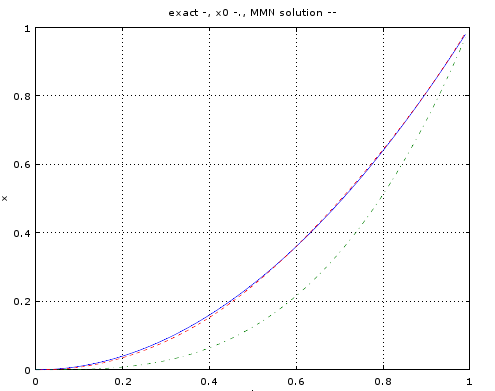
\includegraphics[height=14.0cm]{mmn2_ch1}
	\caption{Восстановленное ММН решение.}
	\label{fig:mmn_ch1}
\end{figure}
Ниже в таблице \ref{table1.1} показаны результаты расчетов методами $\eqref{equ_rmn}$, $\eqref{equ_alphaproc}$, $\Delta=\frac{\|F(x^k)+\alpha(x^k-x^0)-y\|}{\|y\|}$ --- относительная норма невязки. 
\begin{table}[h]
	\centering
	\renewcommand{\arraystretch}{1.5}
	\caption{Результаты для правой части без шума}
	\label{table1.1}
	\begin{tabular}{|l|c|c|c|}
		\hline
	\textbf{Метод}                   & \multicolumn{1}{l|}{\textbf{Параметр шага, $\gamma$}} & \multicolumn{1}{l|}{\textbf{$\Delta$}} & \multicolumn{1}{l|}{\textbf{Число итераций, N}} \\ \hline
		ММО                              & \begin{tabular}[c]{@{}c@{}}0.5\end{tabular}                                       & 0.003                                   & 25                                     \\ \hline
		\multicolumn{1}{|r|}{ММО модиф.} & 0.5                                                                                                           & 0.003                                   & 22                                     \\ \hline
		МНС                              & 0.001                                                                                                         & 0.003                                   & 283                                    \\ \hline
		МНС модиф.                       & \begin{tabular}[c]{@{}c@{}}0.02 (c 0-й итер.), \\ 0.005 (c 30-й итер.),\\   0.002 (c 32-й итер.)\end{tabular} & 0.003                                   & 32                                     \\ \hline
		ММН                              & 1                                                                                                             & 0.003                                   & 32                                     \\ \hline
		ММН модиф.                       & 1                                                                                                             & 0.003                                   & 27                                     \\ \hline
		РМН                              & 1                                                                                                             & 0.003                                   & 26                                     \\ \hline
		РМН модиф.                       & \begin{tabular}[c]{@{}c@{}}0.75\end{tabular}                                       & 0.003                                   & 6                                      \\ \hline
	\end{tabular}
\end{table}

{\bfseries\large Вывод.} Выбор начального приближения, достаточно близкого к точному решению, обусловлен условиями теорем 1.1, 1.5 для сходимости немодифицированных вариантов методов $\eqref{equ_rmn}$, $\eqref{equ_alphaproc}$. Так же следует отметить, что теорема 1.5 не гарантирует, что при $\gamma=1$ итерационный процессы $\eqref{equ_alphaproc}$ будут сходиться, так же как и модифицированный вариант метода Ньютона. Поэтому сходимость некоторых этих методов в рамках эксперимента была достигнута при выборе $\gamma<1$, тогда как для метода Ньютона немодифицированного варианта сходимость при $\gamma=1$ доказана теоремой 1.1, что и подтверждается экспериментом. Для достижения необходимой точности решения модифицированным вариантом МНС параметр $\gamma$ потребовалось несколько раз уменьшать. С 30-й итерации $\gamma=0.005$, с 32-й итерации $\gamma=0.002$.

{\bfseries 1.3.2. Эксперимент для задачи без использования шума с начальным приближением, далеким от точного решения.} 

Точное решение и правая часть такие же, как в эксперименте 1.3.1.  Начальное приближение $x^0(t)=0$, $\bar\alpha=\alpha=10^{-2}$, критерий останова $\frac{\|x^k-z\|}{\|z\|}\le\varepsilon=10^{-1}$, где $x^k$ --- приближение на $k$-й итерации. %%На рис.~\ref{fig:mmn_ch1_const} изображено восстановленное решение методом ММН. Точное решение отмечено голубым цветом, начальное приближение --- малиновым, ММН --- зеленым. 
%\begin{figure}
%	\centering
%	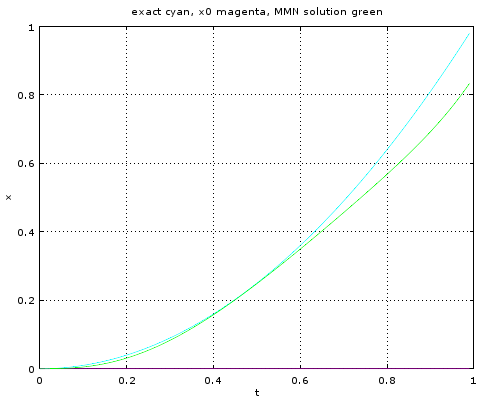
\includegraphics[height=6.0cm]{mmn_ch1_const}
%	\caption{Восстановленное ММН решение с нулевым начальным приближением.}
%	\label{fig:mmn_ch1_const}
%\end{figure}
Ниже в таблице \ref{table1.2} показаны результаты расчетов методами $\eqref{equ_rmn}$, $\eqref{equ_alphaproc}$, $\Delta$ --- относительная норма невязки. 
\begin{table}[h]
	\centering
	\renewcommand{\arraystretch}{1.5}
	\caption{Результаты для правой части без шума, с начальным приближением, равным константе}
	\label{table1.2}
	\begin{tabular}{|l|c|c|c|}
		\hline
		\textbf{Метод}                   & \multicolumn{1}{l|}{\textbf{Параметр шага, $\gamma$}} & \multicolumn{1}{l|}{\textbf{$\Delta$}} & \multicolumn{1}{l|}{\textbf{Число итераций, N}} \\ \hline
		ММО                              & 1                                                     & 0.015                                  & 25                                              \\ \hline
		\multicolumn{1}{|r|}{ММО модиф.} & 0.1                                                   & 0.015                                  & 20                                              \\ \hline
		МНС                              & 0.025                                                 & 0.021                                  & 27                                              \\ \hline
		МНС модиф.                       & 0.025                                                 & 0.024                                  & 24                                              \\ \hline
		ММН                              & 1                                                     & 0.019                                  & 12                                              \\ \hline
		ММН модиф.                       & 1                                                     & 0.016                                  & 8                                               \\ \hline
		РМН                              & 1                                                     & 0.016                                  & 19                                              \\ \hline
		РМН модиф.                       & 0.75                                                  & 0.016                                  & 8                                               \\ \hline
	\end{tabular}
\end{table}

{\bfseries\large Вывод.} Выбор начального приближения обусловлен фактом, установленным в статье \cite{Vasin2016}, где для модифицированных вариантов методов $\eqref{equ_alphaproc}$ доказывается глобальная сходимость итерационных процессов. Для сходимости модифицированного метода Ньютона требование близкого начального приближения оговаривается в статье \cite{VasAkiMin2013}, но в данном случае была достигнута требуемая точность, как и для немодифицированных методов, рассматриваемых в данной главе. Факт сходимости при $\gamma=1$ не установлен для каждого из методов, однако при соответствующем $\gamma<1$ методы $\eqref{equ_rmn}$, $\eqref{equ_alphaproc}$ должны сходиться по теореме 1.5, этому не противоречат результаты расчетов.

\newpage
{\bfseries 1.3.3. Эксперимент для задачи с возмущенной правой частью с начальным приближением, далеким от точного решения.} 

Точное решение такое же, как в эксперименте 1.3.1. Правая часть $y^\delta(t)=y(t)e^{\frac{\delta}{5} sin(t/{\delta}^2)}$, $\delta=0.1$, $\|y-y^{\delta}\|=0.07<\delta$. Начальное приближение $x^0(t)=0$, $\gamma$, $\bar\alpha=1$, $\alpha=10^{-3}$, критерий останова $\frac{\|x^k-z\|}{\|z\|}\le\varepsilon=0.25$, где $x^k$ --- приближение на $k$-й итерации. 

Методы сходятся к $\varepsilon$ за 8--9 итераций, $\Delta\approx 0.04$.
%Ниже в таблице \ref{table1.3} приведены результаты расчетов.
%\begin{table}[H]
%	\centering
%%	\renewcommand{\arraystretch}{1.5}
%	\caption{Результаты для задачи с шумом}
%	\label{table1.3}
%	\begin{tabular}{|l|c|c|}
%		\hline
%		\textbf{Метод}                   & \multicolumn{1}{l|}{\textbf{$\Delta$}} & \multicolumn{1}{l|}{\textbf{Число итераций, N}} \\ \hline
%		ММО                              & 0.042                                  & 9                                               \\ \hline
%		\multicolumn{1}{|r|}{ММО модиф.} & 0.042                                  & 9                                               \\ \hline
%		МНС                              & 0.041                                  & 9                                               \\ \hline
%		МНС модиф.                       & 0.040                                  & 9                                               \\ \hline
%		ММН                              & 0.045                                  & 9                                               \\ \hline
%		ММН модиф.                       & 0.045                                  & 9                                               \\ \hline
%		РМН                              & 0.042                                  & 9                                               \\ \hline
%		РМН модиф.                       & 0.042                                  & 8                                               \\ \hline
%	\end{tabular}
%\end{table}

В статье \cite{VasSkur2017} приводятся оценки погрешности двухэтапного метода для $\|u^{\delta}-\hat{u}\|$ сверху ($u^{\delta}$ --- решение уравнения с возмущенной правой частью, $\hat{u}$ --- решение уравнения $\eqref{equ1}$), устанавливается сходимость $$\lim_{\delta\to 0}\|A(u_{\alpha(\delta)}^{\delta})-f_\delta\|=0,$$ при $\alpha(\delta)\to 0$, $\delta\to 0$. 

{\bfseries\large Вывод.} Для задачи с возмущенной правой частью удалось достигнуть точности $\varepsilon$, не превыщающую оценку для $\|u^{\delta}-\hat{u}\|$, относительная норма невязки $\Delta$ уменьшается с каждой итерацией. 

%\section{Выводы к первой главе}
%% Глава 2
\chapter{Решение уравнений с немонотонным оператором}
Монотонность оператора $A$ исходного уравнения --- очень сильное требование, которое не выполняется во многих важных прикладных задачах, например, в задачах гравиметрии и магнитометрии. В данной главе показано, что в конечномерном случае есть возможность ослабить условие монотонности и обосновать сходимость итераций методов РМН, ММО, МНС, ММН.
В первом параграфе представлены доказательства сходимости метода Ньютона с регуляризацией, во втором параграфе доказаны теоремы сходимости для нелинейных аналогов $\alpha$-процессов, в третьем параграфе представлены следствия для модифицированных аналогов $\alpha$-процессов и оценка невязки двухэтапного метода, в четвертом приведены результаты численного моделирования.

\newpage
\section{Метод Ньютона}
Рассматривается конечномерный случай, когда оператор $A\colon \mathbb{R^n} \to \mathbb{R^n}$, для которого матрица $A'(u)$ в некоторой окрестности решения имеет спектр, состоящий из различных неотрицательных собственных значений.
Приведем лемму (В.В. Васин, \cite{VasSkur2017}).
\begin{lemma}\label{lemVas}
	Пусть $n\times n$ матрица $A'(u)$ не имеет кратных собственных значений $\lambda _i$ и числа $\lambda _i$ ($i=1,2,..n$) различны и неотрицательны. Тогда при $\bar\alpha>0$ матрица имеет представление $A'(u)+\bar\alpha I =S(u)\Lambda S^{-1}(u)$ и справедлива оценка
	\begin{equation}\label{est4.1}
	\|(A'(u)+\bar\alpha I)^{-1}\|\le \frac{\mu (S(u))}{\bar\alpha+\lambda_{min}} \le \frac{\mu(S(u))}{\bar\alpha},
	\end{equation}
	где столбцы матрицы $S(u)$ составлены из собственных векторов матрицы $A'(u)+\bar\alpha I$, $\Lambda$ --- диагональная матрица, ее элементы --- собственные значения матрицы $A'(u)+\bar\alpha I$, $\mu(S(u))=\|S(u)\|\cdot\|S^{-1}(u)\|$. $\square$
\end{lemma}
Обратимся к регуляризованному методу Ньютона, для которого была доказана теорема $\ref{teo2.3}$ о сходимости итераций и оценке погрешности для монотонного оператора. Рассмотрим теперь вариант этой теоремы, когда оператор $A\colon \mathbb{R^n} \to \mathbb{R^n}$, матрица производной $A'(u)$ которого имеет неотрицательный спектр, удовлетворяющий условиям леммы $\ref{lemVas}$, причем функция $\mu(S(u))$ при фиксированном $\alpha$ равномерно ограничена по $u$ в шаре $S(u_\alpha, r)$, т.е.
\begin{equation}\label{cond4.3}
\sup\{\mu(S(u)): u\in S(u_\alpha, r)\}\le\bar S <\infty .
\end{equation}
\begin{theorem}\label{teo4.1}
	Пусть выполнены условия $\eqref{cond4.3}$, $\eqref{cond1.1}$--$\eqref{cond1.3}$, $A'(u^0)$ --- симметричная матрица, и для параметров $\alpha$, $\bar{\alpha}$, $r$ справедливы соотношения: $0<\alpha\le\bar\alpha$, $\bar\alpha\ge 4N_0$, $r\le\alpha/8N_2\bar S$, $\|u_\alpha-u^0\|\le r$.
	Тогда для метода $\eqref{equ_rmn}$ справедливо заключение теоремы $\ref{teo2.3}$, где соотношения $\eqref{ineq2.12}$, $\eqref{eq2.13}$ для $\gamma$ и выражение для $q$ в $\eqref{est2.16}$ соответственно принимает вид
	$$\gamma < \frac{\alpha\bar\alpha}{2(N_1+\alpha)^2\bar S^2}, \quad \gamma _{opt}=\frac{\alpha\bar\alpha}{4(N_1+\alpha)^2\bar S^2}, \quad q=\sqrt{1-\frac{\alpha ^2}{16(N_1+\alpha)^2\bar S^2}}$$
\end{theorem}
\begin{proof} С учетом оценки $\eqref{est4.1}$, доказательство с несущественными поправками проводится по схеме доказательтства теоремы $\ref{teo2.3}$.
\end{proof}

{\remark При доказательстве теоремы вместо условия  $\eqref{cond4.3}$ достаточно требовать ограниченность величины $\sup\{\mu(S(u^k)): u^k \in S(u_\alpha, r)\}$, где $u^k$ --- итерационные точки метода. Причем, при регулярном правиле останова итераций $k(\delta)$, супремум берется по конечному набору номеров $k\le k(\delta)$, что автоматически влечет ограниченность супремума и выполнение оценки вида $\eqref{est2.16}$ при этих значениях $k$. %Кроме того, для модифицированного метода Ньютона, в котором производная $A'(u^0)$ вычисляется в фиксированной точке $u^0$, величина $\mu(S(u^0))=\|S(u^0)\|\|S^{-1}(u^0)\|=\bar S<\infty$.
	}

\newpage
\section{Нелинейные аналоги альфа-процессов}
При тех же условиях на оператор, что и для метода Ньютона в параграфе 2.1, исследуем процессы $\eqref{equ_alphaproc}$.
\begin{theorem}\label{teo4.2}
	Пусть выполнены условия $\eqref{cond1.1}$--$\eqref{cond1.3}$. Пусть при $u \in S(u^0, r)$ матрица $A'(u)$ имеет спектр, состоящий из неотрицательных различных собственных значений, $A'(u^0)$ --- симметричная неотрицательно определенная матрица. Пусть параметры $\alpha$, $\bar{\alpha}$, $r$ удовлетворяют условиям: 
	\begin{equation}\label{cond4.4}
	MMO:\qquad 0<\alpha\le\bar\alpha, \quad r\le\alpha /6\bar SN_2, \quad \bar\alpha \ge N_0
	\end{equation}
	\begin{equation}\label{cond4.5}
	MHC:\qquad 0<\alpha\le\bar\alpha, \quad r\le\alpha /3N_2,
	\end{equation}
	\begin{equation}\label{cond4.6}
	MMH:\qquad 0<\alpha\le\bar\alpha, \quad r\le\alpha /6N_2.
	\end{equation}
	Тогда справедливы соотношения  $\eqref{ineq3.4}$, где
	\begin{equation}\label{eq4.7}
	\mu _{-1}=\frac{8\bar S^2(N_1+\alpha)^2}{\alpha\bar\alpha}, \quad \mu _0=\frac{18(N_1+\alpha)^2(N_1+\bar\alpha)}{\alpha\bar\alpha ^2}, \quad \mu _1=\frac{18(N_1+\alpha)^2(N_1+\bar\alpha)^4}{\alpha\bar\alpha ^5}
	\end{equation}
\end{theorem}
\begin{proof} При $\varkappa=-1$ и тех же обозначениях, которые были приняты в разделе 3, получим (нижний индекс (-1) соответствует методу $\eqref{equ_alphaproc}$ при $\varkappa=-1$)
$$\langle F_{-1}(u), u-u_\alpha\rangle=\beta _{-1}(u)[\langle A(u)-A(u_\alpha), u-u_\alpha\rangle+\alpha\|u-u_\alpha\|^2].$$
Оценим каждое из слагаемых в правой части равенства с учетом условий $\eqref{cond4.4}$, используя формулу Лагранжа
$$\langle A(u)-A(u_\alpha), u-u_\alpha\rangle+\alpha\|u-u_\alpha\|^2=\alpha\|u-u_\alpha\|^2$$ $$+\langle \int\limits_0^1 (A'(u_\alpha+\theta(u-u_\alpha))-A'(u^0))(u-u_\alpha)d\theta, u-u_\alpha\rangle+\langle A'(u^0)(u-u_\alpha), u-u_\alpha\rangle$$ $$\ge \alpha\|u-u_\alpha\|^2-\frac{N_2(\|u^0-u_\alpha\|+\|u-u^0\|)^2}{2}\|u-u_\alpha\|^2$$
\begin{equation}\label {est4.8}
\ge\left ( \alpha-\frac{3N_2 r}{2}\right )\|u-u_\alpha\|^2\ge\frac{3\alpha}{4}\|u-u_\alpha\|^2
\end{equation}
$$\beta _{-1}(u)=\frac{\langle (A'(u)+\bar\alpha I)^{-1}S_\alpha(u), S_\alpha(u)\rangle}{\|S_\alpha(u)\|^2}=\frac{\langle (A'(u^0)+\bar\alpha I)^{-1}S_\alpha(u), S_\alpha(u)\rangle}{\|S_\alpha(u)\|^2}$$ $$+\frac{\langle (B^{-1}(u)-B^{-1}(u^0))S_\alpha(u), S_\alpha(u)\rangle}{\|S_\alpha(u)\|^2}\ge\frac{1}{N_0+\bar\alpha}-\frac{\bar S N_2\|u-u^0\|}{\bar\alpha^2}$$
\begin{equation}\label{est4.9}
\ge\frac{1}{N_0+\bar\alpha}-\frac{2\bar S N_2 r}{\bar\alpha^2}\ge\frac{1}{6\bar\alpha},
\end{equation}
где учтены условия $\eqref{cond4.4}$ и соотношение $\|u-u^0\|\le\|u-u_\alpha\|+\|u_\alpha-u^0\|\le 2r$.

Кроме того, справедлива оценка
$$\|F_{-1}(u)\|^2\le(\beta_{-1}(u))^2\|A(u)-A(u_\alpha)+\alpha(u-u_\alpha)\|^2$$
\begin{equation}\label{est4.10}
\le\|B^{-1}(u)\|^2(N_1+\alpha)^2\|u-u_\alpha\|^2\le\frac{\bar S^2(N_1+\alpha)^2}{\bar\alpha^2}\|u-u_\alpha\|^2
\end{equation}
Объединяя $\eqref{est4.8}$--$\eqref{est4.10}$, получаем, что в соотношении $\eqref{ineq3.4}$, $\mu_{-1}$ выражается величиной из $\eqref{eq4.7}$

Исследуем теперь МНС, т.е. процесс $\eqref{equ_alphaproc}$ при $\varkappa=0$. Аналогично предыдущему методу устанавливаем, что
\begin{equation}\label{est4.11}
\langle A(u)-A(u_\alpha), u-u_\alpha\rangle+\alpha\|u-u_\alpha\|^2\ge\left(\alpha-\frac{3N_2 r}{2}\right)\|u-u_\alpha\|^2
\end{equation}
Кроме того,
$$\beta_0(u)=\frac{\|S_\alpha(u)\|^2}{\langle B(u)S_\alpha(u), S_\alpha(u)\rangle}\ge\frac{1}{\|B(u)\|}\ge\frac{1}{\|A'(u)+\bar\alpha I\|}\ge\frac{1}{N_1+\bar\alpha}.$$
Объединяя последнее соотношение с $\eqref{est4.11}$, получаем оценку снизу
\begin{equation}\label{est4.12}
\langle F_0(u), u-u_\alpha\rangle\ge\frac{1}{N_1+\bar\alpha}\left (\alpha -\frac{3N_2 r}{2}\right )\|u-u_\alpha\|^2.
\end{equation}
Аналог оценки $\eqref{est4.10}$ для $F_0(u)$ следует из неравенств ниже:
\begin{equation}\label{est4.13}
\|F_0(u)\|\le\beta_0(u)(\|A(u)-A(u_\alpha)\|+\alpha\|u-u_\alpha\|)\le\beta_0(u)(N_1+\alpha)\|u-u_\alpha\|,
\end{equation}
$$\beta_0(u)=\frac{\|S_\alpha(u)\|^2}{\bar\alpha\|S_\alpha(u)\|^2+\langle A'(u^0)S_\alpha(u), S_\alpha(u)\rangle+\langle (A'(u)-A'(u^0))S_\alpha(u), S_\alpha(u)\rangle}$$
$$\le \frac{\|S_\alpha(u)\|^2}{\bar\alpha\|S_\alpha(u)\|^2-|\langle (A'(u)-A'(u^0))S_\alpha(u), S_\alpha(u)\rangle|}$$
\begin{equation}\label{est4.14}
\le\frac{1}{\bar\alpha -N_2\|u-u^0\|}\le\frac{1}{\bar\alpha -2N_2 r}
\end{equation}
Из $\eqref{est4.12}$-$\eqref{est4.14}$ при значениях параметров из $\eqref{cond4.5}$ получаем значения $\mu_0$ в $\eqref{eq4.7}$.

Наконец рассмотрим процесс $\eqref{equ_mmn}$ при $\varkappa=1$. Как и в предыдущем методе, при оценке снизу величины $\langle F_1(u), u-u_\alpha\rangle$, справедливо соотношение $\eqref{est4.11}$. Для параметра $\beta_1(u)$ получаем
$$\beta_1(u)=\frac{\langle B(u)S_\alpha(u), S_\alpha(u)\rangle}{\|B(u)S_\alpha(u)\|^2}$$$$\ge\frac{\langle A'(u^0)S_\alpha(u), S_\alpha(u)\rangle+\bar\alpha\langle S_\alpha(u), S_\alpha(u)\rangle-\|A'(u)-A'(u^0)\|\|S_\alpha(u)\|^2}{(N_1+\bar\alpha)^2\|S_\alpha(u)\|^2}$$$$\ge\frac{\bar\alpha -N_2\|u-u^0\|}{(N_1+\bar\alpha)^2}\ge\frac{\bar\alpha -2N_2 r}{(N_1+\bar\alpha)^2},$$
что при условиях на параметры $\eqref{cond4.6}$, дает оценку
\begin{equation}\label{est4.15}
\langle F_1(u), u-u_\alpha\rangle\ge\left (\alpha -\frac{3N_2 r}{2}\right )\frac{\bar\alpha - 2N_2 r}{(N_1+\bar\alpha)^2}\|u-u_\alpha\|^2\ge\frac{\alpha\bar\alpha}{2(N_1+\bar\alpha)^2}\|u-u_\alpha\|^2.
\end{equation}

Поскольку
$$\|F_1(u)\|\le\beta_1(u)(\|A(u)-A(u_\alpha)\|+\alpha\|u-u_\alpha\|)\le \beta_1(u)(N_1+\alpha)\|u-u_\alpha\|,$$ $$\|\beta_1(u)\|\le\frac{(N_1+\bar\alpha)\|S_\alpha(u)\|^2}{\|A'(u)S_\alpha(u)\|^2+2\bar\alpha\langle A'(u)S_\alpha(u), S_\alpha(u)\rangle+\bar\alpha^2\|S_\alpha(u)\|^2}$$ $$\le\frac{(N_1+\bar\alpha)\|S_\alpha(u)\|^2}{2\bar\alpha\langle A'(u^0)S_\alpha(u), S_\alpha(u)\rangle-2\bar\alpha|\langle (A'(u)-A'(u^0))S_\alpha(u), S_\alpha(u)\rangle|+\bar\alpha^2\|S_\alpha(u)\|^2}$$$$
\le\frac{(N_1+\bar\alpha)}{\bar\alpha^2-2\bar\alpha N_2\|u-u^0\|}\le\frac{N_1+\bar\alpha}{\bar\alpha(\bar\alpha - 4N_2 r)}\le\frac{3(N_1+\bar\alpha)}{\bar\alpha^2}.$$
Окончательно получаем для $\|F_1(u)\|^2$ оценку сверху
\begin{equation}\label{est4.16}
\|F_1(u)\|^2\le\frac{3^2(N_1+\alpha)^2(N_1+\bar\alpha)^2}{\bar\alpha^4}\|u-u_\alpha\|^2.
\end{equation}
Объединяя соотношения $\eqref{est4.15}$ и $\eqref{est4.16}$, и условия $\eqref{cond4.6}$, получаем значение $\mu_1$, представленное в $\eqref{eq4.7}$.
\end{proof}
\begin{theorem}\label{teo4.3}
	Пусть выполнены условия теоремы $\ref{teo4.1}$. Тогда при $\gamma<2/\mu _\varkappa$, $\varkappa=-1,0,1$, где значения $\mu _\varkappa$ определяются соотношениями $\eqref{eq4.7}$, последовательности ${u^k}$, порождаемые процессами $\eqref{equ_alphaproc}$, $\eqref{equ_mmn}$ при $\varkappa=-1,0,1$, сходятся к $u_\alpha$, т.е. $$\lim_{k\to\infty}\|u^k-u_\alpha\|=0,$$ а при $
	\gamma{_\varkappa^{opt}}=\frac{1}{\mu_\varkappa}$
	справедлива оценка $\|u^{k+1}-u_\alpha\|\le q{_\varkappa^k}r,$ где
	$$
	q_{-1}=\sqrt{1-\frac{\alpha^2}{64\bar S^2(N_1+\alpha)^2}}, \quad q_0=\sqrt{1-\frac{\alpha^2\bar\alpha^2}{36(N_1+\alpha)^2(N_1+\bar\alpha)^2}},$$
	\begin{equation}\label{eq4.17}
	q_1=\sqrt{1-\frac{\alpha^2\bar\alpha^6}{36(N_1+\alpha)^2(N_1+\bar\alpha)^6}}.
	\end{equation}
\end{theorem}
\begin{proof} Подставляя в соотношение $\eqref{ineq2.20}$ вместо $F(u^k)$ последовательность $F_\varkappa(u^k)$ ($\varkappa=-1,0,1$) и, используя оценки $\eqref{est4.8}$, $\eqref{est4.9}$ ($\varkappa=-1$), $\eqref{est4.9}$, $\eqref{est4.10}$ ($\varkappa=0$), $\eqref{est4.11}$, $\eqref{est4.12}$ ($\varkappa=1$), а также условия на параметры $\eqref{cond4.4}$--$\eqref{cond4.6}$, получаем, после минимизации по $\gamma$, значения для $q_\varkappa$, представленные в $\eqref{eq4.17}$. При выполнении условия $\gamma<2/\mu_\varkappa$, выражение в круглых скобках в правой части неравенства $\eqref{ineq2.20}$ принимает значение, которое меньше единицы, что влечет сходимость итераций для всех трех методов.
\end{proof}

{\remark Предложенный подход к получению оценок скорости сходимости итерационных процессов полностью переносится на случай, когда спектр матрицы $A'(u^k)$, состоящий из различных вещественных значений, содержит набор малых по абсолютной величине отрицательных собственных значений.} 

Пусть $\lambda _1$ --- отрицательное собственное значение с наименьшим модулем $|\lambda_1|$ и $\bar\alpha -|\lambda _1|=\bar\alpha _1<\alpha^*$. Тогда оценка $\eqref{est4.1}$ трансформируется в неравенство
\begin{equation}\label{ineq4.16}
\|(A'(u^k)+\bar\alpha I)^{-1}\|\le\frac{\mu(S(u^k))}{\bar\alpha^*}\le\frac{\bar S}{\bar\alpha^*}
\end{equation}
Все утверждения, т.е. теоремы $(\ref{teo4.1})$--$(\ref{teo4.3})$ остаются справедливыми при замене $\bar\alpha$ на $\bar\alpha^*$ во всех оценках, где используется $\eqref{ineq4.16}$.

{\remark Если рассматривать модифицированные варианты методов $\eqref{equ_rmn}$--$\eqref{equ_mmn}$, когда вместо $A'(u^k)$ в операторе шага используется $A'(u^0)$ в процессе итераций, то при условиях на оператор, принятых в данном разделе, для получения аналогичных результатов о сходимости и оценке погрешности наряду с неотрицательностью спектра достаточно требовать симметричность матрицы $A'(u^0)$ \cite{VasAkiMin2013, Vasin2014, Vasin2016}. Заметим, что при исследовании основных методов $\eqref{equ_rmn}$--$\eqref{equ_mmn}$ существование симметричной матрицы для некоторого элемента $u^0$ предполагается.}

\newpage
\section{Модифицированные варианты регуляризованных методов на основе нелинейных налогов альфа-процессов}
Рассматривается случай, когда производная оператора $A'(u)$ вычисляется в начальной точке итерационных процессов $u^0$. Тогда формулы итерационных процессов $\eqref{equ_alphaproc}$ принимают вид:
%модифицированный метод минимальной ошибки (МММО)
%\begin{equation}\label{m3o}
%u^{k+1}=u^k-\gamma\frac{\langle (A'(u^0)+\bar{\alpha}I)^{-1}S_\alpha(u^k),S_\alpha(u^k)>}{\|S_\alpha(u^k)\|^2}S_\alpha(u^k)\equiv T(u^k),
%\end{equation}
%модифицированный метод наискорейшего спуска (ММНС)
%\begin{equation}\label{m2ns}
%u^{k+1}=u^k-\gamma\frac{\|S_\alpha(u^k)\|^2}{\langle (A'(u^0)+\bar{\alpha}I)S_\alpha(u^k),S_\alpha(u^k)>}S_\alpha(u^k),
%\end{equation}
%модифицированный метод минимальных невязок (МММН)
%\begin{equation}\label{m3n}
%u^{k+1}=u^k-\gamma\frac{\langle (A'(u^0)+\bar{\alpha}I)S_\alpha(u^k),S_\alpha(u^k)>}{\|(A'(u^0)+\bar{\alpha}I)S_\alpha(u^k)\|^2}S_\alpha(u^k).
%\end{equation}
%Все три метода можно кратко записать в виде
\begin{equation}\label{modalphaproc}
u^{k+1}=u^k-\gamma\frac{\langle (A'(u^0)+\bar\alpha I)^{\varkappa}S_\alpha(u^k), S_\alpha(u^k)\rangle}{\langle (A'(u^0)+\bar\alpha I)^{\varkappa+1}S_\alpha(u^k), S_\alpha(u^k)\rangle}S_\alpha(u^k)\equiv T(u^k),
\end{equation}
где при $\varkappa=-1$ итерационный процесс представляет собой модифицированный ММО, при $\varkappa=0$ --- модифицированный МНС и при $\varkappa=1$ --- модифицированный ММН.

Справедлива следующая теорема.
\begin{theorem}\label{teomodalpnomonot}
	Пусть выполнены условия $\eqref{cond1.1}$--$\eqref{cond1.3}$,
$A'(u^0)$ --- самосопряженный оператор, спектр которого состоит из неотрицательных различных собственных значений, параметры $\alpha$, $\bar{\alpha}$, $r$ удовлетворяют условиям
	\begin{equation}\label{cond2.4}
	0\le\alpha\le\bar{\alpha}, \quad r=\alpha/6N_2, \quad \bar{\alpha}\ge N_0.
	\end{equation}
	
	Тогда для оператора
	$$F_\varkappa^0(u)=\beta_{\varkappa}^0(u)S_\alpha(u),$$ где 
	$$\beta_{\varkappa}^0(u)=\frac{\langle (A'(u^0)+\bar\alpha I)^{\varkappa}S_\alpha(u), S_\alpha(u)\rangle}{\langle (A'(u^0)+\bar\alpha I)^{\varkappa+1}S_\alpha(u), S_\alpha(u)\rangle},$$ имеет место неравенство
	$$\|F_\varkappa^0(u)\|^2\le\frac{8(N_1+\alpha)^2}{3\alpha\bar{\alpha}}\langle F_\varkappa^0(u), u-u_\alpha\rangle,$$
	где $\varkappa=-1, 0, 1,$ для модифицированных вариантов ММО, МНС и ММН соответственно.
\end{theorem} 
\begin{proof} Получим оценку снизу скалярного произведения $\langle F_{-1}^0(u),u-u_\alpha\rangle$ для модифицированного ММО.
$$\langle F_{-1}^0(u),u-u_\alpha\rangle=\langle F_{-1}^0(u)-F_{-1}^0(u_\alpha),u-u_\alpha\rangle=\beta_{-1}^0(u)[\langle A(u)-A(u_\alpha),u-u_\alpha\rangle$$ $$+\alpha\|u-u_\alpha\|^2].$$
Оценим снизу $\langle A(u)-A(u_\alpha),u-u_\alpha\rangle$, используя формулу Лагранжа: $$\langle A(u)-A(u_\alpha),u-u_\alpha\rangle=\langle\int_{0}^{1}[A'(u_\alpha+\theta(u-u_\alpha))-A'(u^0)](u-u_\alpha)d\theta, u-u_\alpha\rangle$$ $$+\langle A'(u^0)(u-u_\alpha), u-u_\alpha\rangle\ge-N_2\int_{0}^{1}\|u_\alpha-u^0+\theta(u-u_\alpha)\|\cdot\|u-u_\alpha\|^2d\theta$$ $$=-N_2\|u-u_\alpha\|^2\int_{0}^{1}\|u_\alpha-u^0+\theta u-\theta u_\alpha\pm\theta u^0\|d\theta=-N_2\|u-u_\alpha\|^2$$
$$\times\int_{0}^{1}\|(1-\theta)(u_\alpha-u^0)+\theta(u-u_\alpha)\|d\theta\ge-N_2\|u-u_\alpha\|^2\Big[\int_{0}^{1}(1-\theta)d\theta\cdot\|u^0-u_\alpha\|$$$$+\int_{0}^{1}\theta d\theta\|u-u_\alpha\|^2\Big]=-N_2\|u-u_\alpha\|^2\Big[\frac{\|u_\alpha-u^0\|}{2}+\frac{\|u_\alpha-u^0+u^0-u\|}{2}\Big]$$
\begin{equation}\label{estmodif2.5}
\ge-\frac{3N_2r}{2}\|u-u_\alpha\|^2,
\end{equation}
где $r=\|u_\alpha-u^0\|,\quad \|u-u^0\|\le 2r$.

Получим оценку снизу для множителя $\beta_{-1}^0(u)$, воспользовавшись спектральным разложением резольвенты самосопряженного оператора $A'(u^0)$:
$$\langle (A'(u^0)+\bar{\alpha}I)S_\alpha(u), S_\alpha(u)\rangle=\int_{0}^{N_0}\frac{d\langle E_\lambda S_\alpha(u), S_\alpha(u)\rangle}{\lambda+\bar{\alpha}}\ge\frac{\|S_\alpha(u)\|^2}{N_0+\bar{\alpha}},$$
$$\beta_{-1}^0(u)=\frac{\langle (A'(u^0)+\bar{\alpha}I)S_\alpha(u), S_\alpha(u)\rangle}{\|S_\alpha(u)\|^2}\ge\frac{1}{N_0+\bar{\alpha}}.$$ 
Таким образом, $$\langle F_{-1}^0(u),u-u_\alpha\rangle\ge\frac{1}{N_0+\bar{\alpha}}\Big[\alpha-\frac{3N_2r}{2}\Big]\|u-u_\alpha\|^2.$$
Применяя условия (\ref{cond2.4}) теоремы, получаем оценку
\begin{equation}\label{estmodif2.6}
\langle F_{-1}^0(u),u-u_\alpha\rangle\ge\frac{3\alpha}{8\bar{\alpha}}\|u-u_\alpha\|^2.
\end{equation}
Получим оценку нормы оператора $F_{-1}^0$:
$$\|F_{-1}^0(u)\|=|\beta_{-1}^0(u)|\cdot\|A(u)+\alpha(u-u^0)-f_\delta\|=|\beta_{-1}^0(u)|\cdot\|A(u)-A(u_\alpha)+\alpha(u-u_\alpha)\|.$$
\begin{equation}\label{estmodif2.7}
\|A(u)+\alpha(u-u^0)-f_\delta\|\le(N_1+\alpha)\|u-u_\alpha\|.
\end{equation}
$$\beta_{-1}^0(u)=\frac{1}{\|S_\alpha(u)\|^2}\int_{0}^{N_0}\frac{d\langle E_\lambda S_\alpha(u), S_\alpha(u)\rangle}{\lambda + \bar{\alpha}}\le\frac{1}{\bar{\alpha}},$$
\begin{equation}\label{estmodif2.8}
\|F_{-1}^0(u)\|^2\le\frac{(N_1+\alpha)^2}{\bar{\alpha}^2}\|u-u_\alpha\|^2.
\end{equation}
Объединим (\ref{estmodif2.6}) и (\ref{estmodif2.8}), получаем
$$\|F_{-1}^0(u)\|^2\le\frac{8(N_1+\alpha)^2}{3\alpha\bar{\alpha}}\langle F_{-1}^0(u), u-u_\alpha\rangle$$ для модифицированного варианта ММО.

Рассмотрим модифицированный вариант МНС ($\varkappa=0$).
$$\langle F_0^0(u), u-u_\alpha\rangle=\beta_0^0(u)[\langle A(u)-A(u_\alpha), u-u_\alpha\rangle+\alpha\|u-u_\alpha\|^2].$$
Учитывая, что $\langle (A'(u^0)+\bar{\alpha}I)S_\alpha(u), S_\alpha(u)\rangle\le(N_0+\bar{\alpha})\|S_\alpha(u)\|^2$, имеем
$$\beta_0^0(u)=\frac{\|S_\alpha(u)\|^2}{\langle (A'(u^0)+\bar{\alpha}I)S_\alpha(u), S_\alpha(u)\rangle}\ge\frac{1}{N_0+\bar{\alpha}}.$$
Воспользовавшись ранее полученной оценкой (\ref{estmodif2.5}), имеем
\begin{equation}\label{estmodif2.11}
\langle F_0^0(u), u-u_\alpha\rangle\ge\frac{3\alpha}{8\bar{\alpha}}\|u-u_\alpha\|^2.
\end{equation}
Оценивая сверху $\beta_0^0(u)$ как
\begin{equation}\label{estmodif2.12}
\beta_0^0(u)\le\frac{1}{\bar{\alpha}},
\end{equation}
при объединении неравенств (\ref{estmodif2.7}), (\ref{estmodif2.11}) и (\ref{estmodif2.12}), приходим к соотношению
$$\|F_0^0(u)\|^2\le\frac{8(N_1+\alpha)^2}{3\alpha\bar{\alpha}}\langle F_0^0(u), u-u_\alpha\rangle$$ для модифицированного варианта МНС.

Для модифицированного ММН ($\varkappa=1$), по аналогии, оценим сверху и снизу параметр $\beta_1^0(u)$. Обозначим $B_0(u)=A'(u^0)+\bar{\alpha}I,$
$$\beta_1^0(u)=\frac{\langle B_0(u)S_\alpha(u), S_\alpha(u)\rangle}{\|B_0(u)S_\alpha(u)\|^2}=\frac{\|B_0^{1/2}(u)S_\alpha(u)\|^2}{\|B_0^{1/2}\|^2\|B_0^{1/2}S_\alpha(u)\|^2}\ge\frac{1}{\|B_0(u)\|}\ge\frac{1}{N_0+\bar{\alpha}}.$$
Объединяя эту оценку и оценку (\ref{estmodif2.5}), имеем соотношение
\begin{equation}\label{estmodif2.13}
\langle F_1^0(u), u-u_\alpha\rangle\ge\frac{3\alpha}{8\bar{\alpha}}\|u-u_\alpha\|^2.
\end{equation}
И наконец,
$$\beta_1^0(u)=\frac{\langle B_0(u)S_\alpha(u), S_\alpha(u)\rangle}{\langle B_0(u)S_\alpha(u), A'(u^0)S_\alpha(u)\rangle+\bar{\alpha}\langle B_0(u)S_\alpha(u), S_\alpha(u)\rangle}$$
$$\le\frac{\langle B_0(u)S_\alpha(u), S_\alpha(u)\rangle}{\bar{\alpha}\langle B_0(u)S_\alpha(u), S_\alpha(u)\rangle}=\frac{1}{\bar{\alpha}},$$
так как $$\langle B_0(u)S_\alpha(u), A'(u^0)S_\alpha(u)\rangle=\langle A'(u^0)S_\alpha(u), A'(u^0)S_\alpha(u)\rangle$$$$+\bar{\alpha}\langle S_\alpha(u), A'(u^0)S_\alpha(u)\rangle\ge 0$$ в силу неотрицательности спектра оператора $A'(u^0)$. Таким образом,
\begin{equation}\label{estmodif2.14}
\|F_1^0(u)\|^2\le\frac{(N_1+\alpha)^2}{\bar{\alpha}^2}\|u-u_\alpha\|^2,
\end{equation}
объединяя (\ref{estmodif2.13}), (\ref{estmodif2.14}), получаем
$$\|F_1^0(u)\|^2\le\frac{8(N_1+\alpha)^2}{3\alpha\bar{\alpha}}\langle F_1^0(u), u-u_\alpha\rangle.$$
\end{proof}

Докажем сходимость итераций $\eqref{modalphaproc}$ к регуляризованному решению $u_\alpha$.
\begin{theorem}
	Пусть выполнены условия теоремы \ref{teomodalpnomonot}. Тогда при $\gamma < 2/\mu_\varkappa$ последовательность $\{u^k\}_{k=1}^\infty$ сходится к регуляризованному решению $u_\alpha$: $$\lim\limits_{k\to\infty}\|u^k-u_\alpha\|=0,$$ а при $\gamma_{opt}=1/\mu_\varkappa$ справедлива оценка $\|u^k-u_\alpha\|\le q{_\varkappa^k}r,$ где
	$$q^\varkappa=\sqrt{1-\frac{9\alpha^2}{64(N_1+\alpha)^2}}$$
\end{theorem}
\begin{proof} Неравенства $\eqref{fejer_prop_uni}$, $\eqref{fejer_prop_it}$ будут выполнены при $\mu_\varkappa=\frac{2}{\gamma(1+\nu)}$ (из теоремы~\ref{teomodalpnomonot}), $\nu=\frac{2}{\gamma\mu_\varkappa}-1,$ где $\gamma<2/\mu_\varkappa$. Отсюда следует сходимость итераций к $u_\alpha$.

Величину $q$ получим из условия минимума $\|u^{k+1}-u_\alpha\|^2$:
$$\|u^{k+1}-u_\alpha\|^2=\|u^k-u_\alpha\|^2-2\gamma\langle F_\varkappa(u^k), u^k-u_\alpha\rangle+\gamma^2\|F_\varkappa(u^k)\|^2$$
\begin{equation}\label{estmod2.11}
\le\big(1-2\gamma\frac{3\alpha}{8\bar{\alpha}}+\gamma^2\frac{(N_1+\alpha)^2}{\bar{\alpha}^2}\big)\|u^k-u_\alpha\|^2.
\end{equation}
$$\gamma_{opt}=argmin\{1-2\gamma\frac{3\alpha}{8\bar{\alpha}}+\gamma^2\frac{(N_1+\alpha)^2}{\bar{\alpha}^2}\},$$
подставляя полученное $\gamma_{opt}$ в выражение в круглых скобках~(\ref{estmod2.11}), вычисляем значение для $q^\varkappa$:
$$\|u^{k+1}-u_\alpha\|^2\le\big(1-\frac{9\alpha^2}{64(N_1+\alpha)^2}\big)\|u^k-u_\alpha\|^2,$$ отсюда получаем $q^\varkappa$.
\end{proof}

Для оператора $A'(u)$ с положительным спектром так же, как и для случая монотонного оператора, в главе 2 доказана линейная скорость сходимости, однако, в отличие от монотонного оператора здесь оценок типа $\eqref{est5.2}$ не удалось получить, поэтому нет общей оценки для двухэтапного метода. Тем не менее, в этой ситуации для двухэтапного алгоритма можно установить оценку для невязки --- основной характеристики точности метода при решении задачи с реальными данными.

Предположим, что уравнение $\eqref{equ2}$ разрешимо, тогда для его решения $u_{\alpha(\delta)}^{\delta}$ справедливо соотношение
\begin{equation}\label{equ5.8}
\|A(u_{\alpha(\delta)}^{\delta})-f_\delta\|=\alpha(\delta)\|u_{\alpha(\delta)}^{\delta}-u^0\|.
\end{equation}
Параметр $\alpha$ из $\eqref{equ2}$ заменен на $\alpha(\delta)$, чтобы подчеркнуть зависимость параметра регуляризации от $\delta$.
Пусть для некоторой зависимости $\alpha(\delta)$ ограничена величина $\|u_{\alpha(\delta)}^{\delta}-u^0\|\le m <\infty$, что влечет оценку
\begin{equation}\label{est5.9}
\|A(u_{\alpha(\delta)}^{\delta})-f_\delta\|\le\alpha(\delta)m
\end{equation}
и сходимость $$\lim_{\delta\to 0}\|A(u_{\alpha(\delta)}^{\delta})-f_\delta\|=0,$$ при $\alpha(\delta)\to 0$, $\delta\to 0$. Пусть ${u_{\alpha(\delta)}^{\delta, k}}$ -- итерационные точки, полученные одним из методов $\eqref{equ_rmn}$, $\eqref{equ_alphaproc}$. Имеем
\begin{equation}\label{est5.10}
\|A(u_{\alpha(\delta)}^{\delta, k})-f_\delta\|\le\|A(u_{\alpha(\delta)}^{\delta, k})-A(u_{\alpha(\delta)}^{\delta})\|+\|A(u_{\alpha(\delta)}^{\delta})-f(\delta)\|\le N_1 r q^k(\delta)+\alpha(\delta)m.
\end{equation}
Выбирая, например, $\alpha(\delta)=\delta^p$ и приравнивая слагаемые в правой части $\eqref{est5.10}$, получаем правило выбора числа итерации
$$k(\delta)=\left [\ln(m\delta^p/N_1)/\ln q(\delta)\right ],$$
при котором справедлива оценка для невязки двухэтапного метода (см. статью \cite{VasSkur2017})
\begin{equation}\label{est5.11}
\|A(u_{\alpha(\delta)}^{\delta,k})-f_\delta\|\le 2m\delta^p.
\end{equation}
{\remark Соотношения $\eqref{equ5.8}$--$\eqref{est5.11}$ остаются справедливыми для случая, когда матрицы $A'(u^k)$ содержат набор малых отрицательных собственных значений с тем лишь отличием, что в неравенстве $\eqref{est5.10}$ параметр $q$ во всех методах теперь вычисляется по формулам главы 2, с заменой параметра $\bar\alpha$ зна $\alpha^*$ (см. замечание 2.2).}

\newpage
\section{Решение модельных задач гравиметрии и магнитометрии}

{\bfseries Целью} экспериментов является проверить применимость методов $\eqref{equ_rmn}$, $\eqref{equ_alphaproc}$, $\eqref{equ_mmn}$ с немонотонным оператором на примере решения модельных задач гравиметрии и магнитометрии. Также ставится задача сравнить по экономичности (затратам машинного времени) методы $\eqref{equ_rmn}$, $\eqref{equ_alphaproc}$ с их модифицированными вариантами, когда производная $A'(u^k)$, входящая в оператор шага этих процессов, вычисляется в фиксированной точке $u^0$ в течение всего процесса итераций, т.е. $A'(u^k)$ в $\eqref{equ_rmn}$, $\eqref{equ_alphaproc}$ заменяется на $A'(u^0)$ (см. \cite{Vasin2014, Vasin2016}). 

{\bfseries 2.4.1. Решение структурной обратной задачи гравиметрии} 

Рассматривается трехмерная структурная обратная задача гравиметрии о нахождении поверхностей раздела сред по известному скачку плотности и гравитационному полю, измеренному на некоторой площади земной поверхности.
Рассмотрим уравнение гравиметрии для модели двуслойной среды в декартовой системе координат с осью $z$, направленной вниз 
\begin{equation}\label{equ_grav2l}
\begin{aligned}
g\Delta\sigma\frac{1}{4\pi} \bigg\{ \iint_{D} \frac{1}{[(x-x')^2+(y-y')^2+H^2]^{1/2}}dx'dy' \\
- 
\iint_{D} \frac{1}{[(x-x')^2+(y-y')^2+u^2(x',y')]^{1/2}}dx'dy'\bigg\}=\Delta f(x,y),
\end{aligned} 
\end{equation}
где $g$ --- гравитационная постоянная, $\Delta\sigma=\sigma_2-\sigma_1$ --- скачок плотности на поверхности раздела сред, описываемой функцией $u(x,y)$ и подлежащей определению, $\Delta f(x,y)$ --- аномальное гравитационное поле, вызванное отклонением поверхности от асимптотической плоскости $z=H$ для искомого решения $u(x,y)$ (рис.~\ref{fig:twolayergrav}). 
\begin{figure}[H]
	\centering
	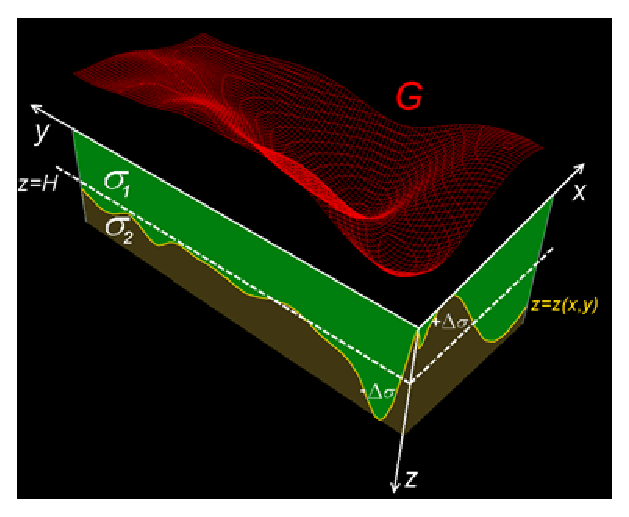
\includegraphics[height=14.0cm]{Twolaymodgrav}
	\caption{Модель двуслойной среды в задаче гравиметрии.}
	\label{fig:twolayergrav}
	\end{figure}
Запишем $\eqref{equ_grav2l}$ в виде операторного уравнения
\begin{equation}\label{equ_2lop}
	[A(u)](x,y)=-\iint_{D} \frac{1}{[(x-x')^2+(y-y')^2+u^2(x',y')]^{1/2}}dx'dy'=f(x,y),
\end{equation}
где $f(x,y)=\Delta f(x,y) 4\pi/g\Delta\sigma - A(H)$. Тогда производная оператора $A$ в точке $u^0(x,y)$ определяется формулой
$$ [A'(u^0)]h=\iint_{D} \frac{u^0(x',y')h(x',y')}{[(x-x')^2+(y-y')^2+(u^0(x',y'))^2]^{3/2}}dx'dy', $$
Уравнение (\ref{equ_2lop}) является интегральным уравнением Урысона (так как неизвестная функция $u(x,y)$ входит в ядро оператора нелинейно) I рода, следовательно, относится к классу некорректных задач.
	
После дискретизации интегрального уравнения $\eqref{equ_2lop}$ двумерным аналогом формулы прямоугольников с равномерной сеткой по каждой переменной с шагом $\Delta x$, $\Delta y$, получаем систему нелинейных уравнений относительно неизвестного вектора $u_{ji}=u(x_j,y_i)\quad (j=1,2,...,N, i=1,2,...,M)$, которая в векторно-матричном виде может быть записана следующим образом
\begin{equation}\label{equ_snle}
	A_n(u_n)=f_n,
\end{equation}
где $u_n$, $f_n$ --- векторы размерности $n=N\times M$. Дискретный аналог производной $A'(u^0)$ принимает форму
\begin{equation}\label{op_grav_disc_form}
	[A'_n(u_n^0)h_n]_{k,l}=\sum\limits_{i=1}^{M}\sum\limits_{j=1}^{N}
	\Delta x\Delta y\frac{u^0_{ji}h_{ji}}{[(x_k-x'_j)^2+(y_l-y'_i)^2+(u^0_{ji})^2]^{3/2}},
\end{equation}
где при $u_{n}^{0}=const$ матрица $A'_n(u_n^0)$ симметрична, элементы которой вычисляются по формуле $\eqref{op_grav_disc_form}$.

Рассматривается модель двухслойной среды, в которой поверхность раздела задается функцией $u(x,y)$, по формуле %\cite{AkMisSkurTre2015_1}
$$
\hat{u}(x,y)=5-3.21e^{-(x/10.13-6.62)^6-(y/9.59-2.93)^6}-
2.78e^{-(x/9.89-4.12)^6-(y/8.63-7.43)^6}$$
\begin{equation}\label{form6.5}
+3.13e^{-(x/9.89-4.82)^6-(y/8.72-4.33)^6},
\end{equation}
заданной в области $D=\{0\le x\le 100, 0\le y \le 110\}$. Была выбрана сетка с шагом $\Delta x=\Delta y=1$ (км), что приводит к размерности $n=11000$ для искомого вектора $u_n$, а также принято, что $\Delta\sigma=0.21$ (г/см$^3$), $H=5$ (км) ($z=H=5$ --- асимптотическая плоскость для $\hat{u}(x,y)$).

В результате численного эксперимента по восстановлению модельного решения $\eqref{form6.5}$ было установлено, что не только матрица $A'_n(u^0)$ имеет $n$ различных неотрицательных собственных значений, но это свойство имело место и для $A'(u_n^k)$ на каждой $k$-итерации. Тем самым выполнены условия, при которых получены результаты в данной главе по сходимости и оценке погрешности процессов $\eqref{equ_rmn}$, $\eqref{equ_alphaproc}$ для немонотонного оператора $A$ с положительным спектром. 

При анализе числа обусловленности $\mu(A'_n(u_n^k))$ было установлено, что эта величина для всех четырех процессов принимала значения $\mu(A'_n(u_n^k))\approx 4.6 * 10^{8}$ для немодифицированного варианта и $\mu(A'_n(u_n^0))\approx 1.5 * 10^{4}$ для модифицированных методов. Выход из процесса итераций каждого из методов осуществлялся по правилу
\begin{equation}\label{cond6.6}
\frac{\|\hat{u}_n-\tilde{u}_n\|_{R^n}}{\|\tilde{u}_n\|_{R^n}}\le\varepsilon=10^{-2},
\end{equation}
где $\hat{u}_n$ --- точное решение системы уравнений $\eqref{equ_snle}$, а $\tilde{u}_n$ --- восстановленное каждым из четырех итерационных методов.

В таблице $\ref{Table_gravy}$ представлены результаты расчетов при значениях параметров $\bar\alpha=\alpha=10^{-3}$, $\gamma=1$, где
\begin{equation}\label{form6.7}
\Delta=\frac{\|A_n(\tilde{u}_n)+\alpha(\tilde{u}_n-u^0)-f_n\|_{R^n}}{\|f_n\|_{R^n}},
\end{equation}
относительная регуляризованная невязка для восстановленного решения, $N_\varepsilon$ --- число итераций в процессе для достижения точности, определяемой неравенством $\eqref{cond6.6}$, $T$ --- время реализации метода. В позициях для $\Delta$, $N_\varepsilon$, $T$ верхняя строка соответствует основным процессам, а нижняя --- их модифицированным вариантам.
\begin{table}[H]
	\centering
	\renewcommand{\arraystretch}{1.5}
	\caption{Эксперименты для обратной задачи гравиметрии}
	\label{Table_gravy}
	\begin{tabular}{|p{0.2\textwidth}|p{0.1\textwidth}|p{0.1\textwidth}|p{0.1\textwidth}|p{0.1\textwidth}|}
		\hline
		\rule{0cm}{0.5cm}
		\textbf{Методы} & \textbf{ММО} & \textbf{МНС} & \textbf{ММН} & \textbf{РМН} \\ \hline
		\rule{0cm}{0.5cm}
		{$\Delta$} & 0.0048 & 0.0020 & 0.0024 & 0.0023	 \\ \cline{2-5} 
		\rule{0cm}{0.5cm}
		&  0.0094   & 0.0019    &  0.0019   &  0.0021   \\ \hline
		\rule{0cm}{0.5cm}
		{$N_\varepsilon$} & 17  &  21   &   20  &  16    \\ \cline{2-5}
		\rule{0cm}{0.5cm}
		&  22   &   23  &  23   &  16   \\ \hline
		\rule{0cm}{0.5cm}
		{$T$ (сек)}    &  30   &  11   &  14  & 27    \\ \cline{2-5}
		\rule{0cm}{0.5cm}
		& 35   & 12    &  15   &   26  \\ \hline
	\end{tabular}
\end{table}

{\bfseries 2.4.2. Решение структурной обратной задачи магнитометрии}
 
Уравнение магнитометрии при тех же предположениях, что и в задаче гравиметрии для двухслойной среды, имеет вид
\begin{equation}\label{equ_magn}\begin{aligned}
\Delta J  \bigg\{&\iint_{D} \frac{H}{[(x-x')^2+(y-y')^2+H^2]^{3/2}}dx'dy' \\
- &\iint_{D} \frac{u(x',y')}{[(x-x')^2+(y-y')^2+u^2(x',y')]^{3/2}}dx'dy' \bigg\}=\Delta G(x,y),
\end{aligned} \end{equation}
где $\Delta J$ --- усредненный скачок $z$-компоненты вектора намагниченности, $z=H$ --- асимптотическая плоскость, $u(x,y)$ --- функция, описывающая аномальное поле, $z=u(x,y)$ --- искомая функция, описывающая поверхность раздела сред с различными свойствами намагниченности (рис.~\ref{fig:twolayermag}). 
\begin{figure}[H]
	\centering
	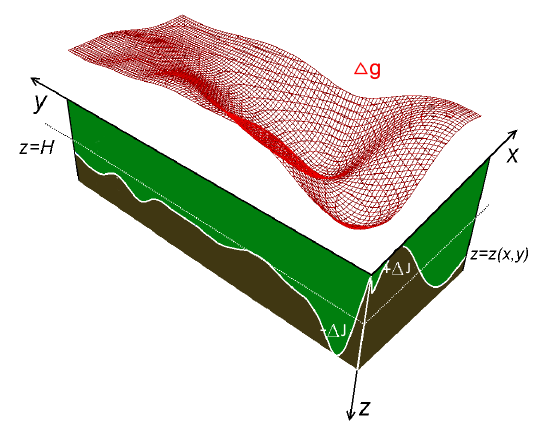
\includegraphics[height=14.0cm]{Twolaymodmag}
	\caption{Модель двуслойной среды в задаче магнитометрии.}
	\label{fig:twolayermag}
\end{figure}
Уравнение $\eqref{equ_magn}$ можно переписать в форме
\begin{equation}\label{equ_magn_op}
[D(u)](x,y)= \iint_{D} \frac{u(x',y')}{[(x-x')^2+(y-y')^2+u^2(x',y')]^{3/2}}dx'dy'=F(x,y),
\end{equation}
где $F(x,y)=D(H)-\Delta G(x,y)/\Delta J$, тогда производная оператора $D$ в точке $u^0(x,y)$ определится формулой
$$ [A'(u^0)]h=\iint_{D} \frac{(x-x')^2+(y-y')^2-2(u^0(x',y'))^2}{[(x-x')^2+(y-y')^2+(u^0(x',y'))^2]^{5/2}}h(x',y')dx'dy'. $$

После дискретной аппроксимации, подобно задаче гравиметрии уравнения $\eqref{equ_magn_op}$, приходим к системе нелинейных уравнений
\begin{equation}\label{equ_snle_mag}
D_n(u_n)=F_n
\end{equation}
относительно вектора $u_n \quad (n=N\times M)$ с компонентами $u_{ij}\quad (i=1,2,...,N, j=1,2,...,M)$, при этом компоненты производной оператора $D_n$ в точке $u_{n}^{0}$ вычисляются по формуле
\begin{equation}\label{deriv_op_mag}
[D'_n(u_{n}^{0})h_n]_{k,l}=\sum\limits_{i=1}^{N}\sum\limits_{j=1}^{M}
\Delta x\Delta y\frac{(x_k-x'_j)^2+(y_l-y'_i)^2-2(u_{ji}^0)^2}{[(x_k-x'_j)^2+(y_l-y'_i)^2+(u_{ji}^0)^2]^{5/2}}h_{ji}, 
\end{equation}
причем при $u_{n}^{0}=\{u^0(x'_j, y'_i), 1\le j\le M, 1\le i\le N\}=const$, $D'_n(u_n^0)$ --- симметричная матрица.

Модельное решение уравнения $\eqref{equ_snle_mag}$, определяющее поверхность раздела сред, задается формулой \cite{AkMisDer2014}
\begin{equation}\label{form6.11}
\hat{u}(x,y)=5-2e^{-(x/10-3.5)^6-(y/10-2.5)^6}-
3^{-(x/10-5.5)^6-(y/10-4.5)^6},
\end{equation}
на области $D=\{0\le x \le 100, 0\le y\le 100\}$. Сетка строилась с шагом $\Delta x=\Delta y = 1$ (км), что влечет размерность $n=10000$ для искомого вектора $u_n$.

Для $\Delta J=0.4$  был выполнен численный эксперимент по восстановлению модельного решения задачи $\eqref{equ_magn_op}$ процессами $\eqref{equ_rmn}$, $\eqref{equ_alphaproc}$ при $\bar\alpha=0.01$, $\alpha = 0.0001$, $\beta=1$, а также их модифицированными аналогами, когда производная $D'(u^k)$ вычисляется в фиксированной точке $u_n^0=H=5$ (км). Число обусловленности $\mu(D'_n(u_n^0))=1.8\cdot 10^7$. После вычисления спектра матрицы $D'_n(u_n^k)$ выяснилось, что она имеет различные неотрицательные собственные значения, что на основании теорем сходимости главы 2, при подходящем выборе параметра $\beta$ и начальном приближении $u_n^0$, гарантирует сходимость итерационных схем и двухэтапного метода. Окончание итерационных процессов выполнялось по правилу $\eqref{cond6.6}$.

Результаты расчетов для задачи $\eqref{equ_snle_mag}$ по восстановлению модельного решения $\eqref{form6.11}$ представлены в таблице $\ref{Table_magne}$. Как и в таблице $\ref{Table_gravy}$, здесь $\Delta$ --- относительная норма невязки $\eqref{form6.7}$ для восстановленного решения, $N_\varepsilon$ --- число итераций для достижения точности $\eqref{cond6.6}$, $T$ --- машинное время при реализации процесса, верхние строки для каждого параметра соответствуют данным для основных (немодифицированных) процессов $\eqref{equ_rmn}$, $\eqref{equ_alphaproc}$, $\eqref{equ_mmn}$, нижние строки --- для модифицированных методов $\eqref{modalphaproc}$.
\begin{table}[H]
	\centering
%	\renewcommand{\arraystretch}{1.5}
	\caption{Эксперименты для обратной задачи магнитометрии}
	\label{Table_magne}
	\begin{tabular}{|p{0.2\textwidth}|p{0.1\textwidth}|p{0.1\textwidth}|p{0.1\textwidth}|p{0.1\textwidth}|}
		\hline
		\rule{0cm}{0.5cm}
		\textbf{Методы} & \textbf{ММО} & \textbf{МНС} & \textbf{ММН} & \textbf{РМН} \\ \hline
		\rule{0cm}{0.5cm}
		{$\Delta$} & 0.0636 & 0.0699 & 0.0802 & 0.0368	 \\ \cline{2-5} 
		\rule{0cm}{0.5cm}
		&  0.0569   & 0.0575    &  0.0595   &  0.0369   \\ \hline
		\rule{0cm}{0.5cm}
		{$N_\varepsilon$} & 4  &  4   &   4  &  5    \\ \cline{2-5}
		\rule{0cm}{0.5cm}
		&  4   &   4  &  4   &  5   \\ \hline
		\rule{0cm}{0.5cm}
		{$T$ (сек)}    &  7   &  6   &  6  & 22    \\ \cline{2-5}
		\rule{0cm}{0.5cm}
		& 5    & 3    &  3   &   3  \\ \hline
	\end{tabular}
\end{table}

{\bfseries\large Вывод.} Анализируя результаты численного эксперимента для задач гравиметрии и магнитометрии, можно отметить, что для достижения одной и той же точности приближенного решения в соответствии с правилом $\eqref{cond6.6}$, число итераций для модифицированных методов, как правило, больше, чем немодифицированных процессов $\eqref{equ_rmn}$, $\eqref{equ_alphaproc}$. Однако затраты машинного времени при реализации модифицированных процессов, за исключением ММО, существенно меньше. Поэтому можно сделать вывод, что модифицированные МНС, ММН и РМН более экономичны и, следовательно, более предпочтительны для некоторых классов нелинейных задач большой размерности. Более затратная по времени реализация ММО, по сравнению с МНС и ММН, связана прежде всего с тем, что в коэффициенте $\beta_{-1}(u^k)$ необходимо вычислять не только скалярные произведения, но и обращать на каждом шаге оператор $B_k=A'(u^k)+\alpha I$. Следует сказать, что для уравнения $\eqref{equ1}$ ММО обычно не используется. Его применение целесообразно для эквивалентного уравнения $A'(u)^*(A(u)-f)=0$, для которого ММО преобразуется к виду, где операция обращения отсутствует [\cite{VasEre2009},	c.~57, формула 5.8]. Заметим также, что в методе ММО и РМН вычисление элемента вида $W=(A'(u^k)+\alpha I)^{-1}V$ заменялось приближенным решением системы $(A'(u^k)+\alpha I)W=V$ с помощью метода минимальных невязок, т.е. в этом случае фактически реализуется гибридная схема градиентно--ньютоновского типа. 

Как можно видеть из таблицы $\ref{Table_magne}$, также тенденция по затратам машинного времени для модифицированных процессов $\eqref{modalphaproc}$ (включая ММО) также сохраняется и для обратной задачи магнитометрии. 


%\section{Выводы ко второй главе}
%% Глава 3
\chapter{Покомпонентные методы и вычислительные оптимизации}

%\section{Постановки задач}

%Рассматривается трехмерная структурная обратная задача гравиметрии о нахождении поверхностей раздела сред по известным скачкам плотности и гравитационному полю, измеренному на некоторой площади земной поверхности.
%Рассмотрим уравнение гравиметрии для модели двуслойной среды в декартовой системе координат с осью $z$, направленной вниз 
%\begin{equation}\label{equ_grav2l}
%\begin{aligned}
%\gamma\Delta\sigma\frac{1}{4\pi} \bigg\{ \iint_{D} \frac{1}{[(x-x')^2+(y-y')^2+H^2]^{1/2}}dx'dy' \\
%- 
%\iint_{D} \frac{1}{[(x-x')^2+(y-y')^2+u^2(x',y')]^{1/2}}dx'dy'\bigg\}=\Delta g(x,y),
%\end{aligned} 
%\end{equation}
%где $\gamma$ --- гравитационная постоянная, $\Delta\sigma=\sigma_2-\sigma_1$ --- скачок плотности на поверхности раздела сред, описываемой функцией $u(x,y)$ и подлежащей определению, $f(x,y)$ --- аномальное гравитационное поле, вызванное отклонением поверхности от асимптотической плоскости $z=H$ для искомого решения $u(x,y)$ (рис.~\ref{fig:twolayergrav}). 
%\begin{figure}
%	\centering
%	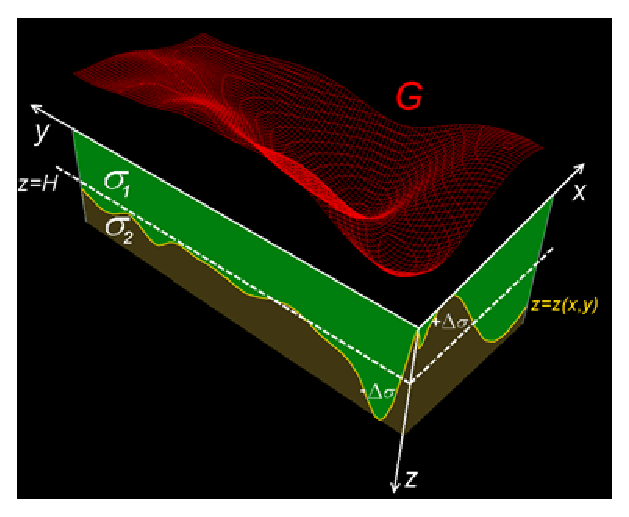
\includegraphics[height=6.0cm]{Twolaymodgrav}
%	\caption{Модель двуслойной среды в задаче гравиметрии.}
%	\label{fig:twolayergrav}
%\end{figure}
%Запишем $\eqref{equ_grav2l}$ в виде операторного уравнения
%\begin{equation}\label{equ_2lop}
%[A(u)](x,y)=-\iint_{D} \frac{1}{[(x-x')^2+(y-y')^2+u^2(x',y')]^{1/2}}dx'dy'=f(x,y),
%\end{equation}
%где $f(x,y)=\Delta g(x,y) 4\pi/\gamma\Delta\sigma - A(H)$. Тогда производная оператора $A$ в точке $u^0(x,y)$ определяется формулой
%$$ [A'(u^0)]h=\iint_{D} \frac{u^0(x',y')h(x',y')}{[(x-x')^2+(y-y')^2+(u^0(x',y'))^2]^{3/2}}dx'dy', $$
%Уравнение (\ref{equ_2lop}) является интегральным уравнением Урысона (так как неизвестная функция $u(x,y)$ входит в ядро оператора нелинейно) I рода, следовательно, относится к классу некорректных задач.
%
%После дискретизации интегрального уравнения $\eqref{equ_2lop}$ двумерным аналогом формулы прямоугольников с равномерной сеткой по каждой переменной с шагом $\Delta x$, $\Delta y$, получаем систему нелинейных уравнений относительно неизвестного вектора $u_{ji}=u(x_j,y_i)\quad (j=1,2,...,N, i=1,2,...,M)$, которая в векторно-матричном виде может быть записана следующим образом
%\begin{equation}\label{equ_snle}
%A_n(u_n)=f_n,
%\end{equation}
%где $u_n$, $f_n$ --- векторы размерности $n=N\times M$. Дискретный аналог производной $A'(u^0)$ принимает форму
%\begin{equation}\label{op_grav_disc_form}
%[A'_n(u_n^0)h_n]_{k,l}=\sum\limits_{i=1}^{M}\sum\limits_{j=1}^{N}
%\Delta x\Delta y\frac{u^0_{ji}h_{ji}}{[(x_k-x'_j)^2+(y_l-y'_i)^2+(u^0_{ji})^2]^{3/2}},
%\end{equation}
%где при $u_n=u_{n}^{0}$ --- const $A'_n(u_n^0)$ --- симметричная матрица, компоненты которой вычисляются по формуле $\eqref{op_grav_disc_form}$.

%Рассмотрим уравнение гравиметрии для модели многослойной среды. 
%
%Предполагается, что нижнее полупространство состоит из нескольких слоев постоянной плотности $\Delta\sigma_l(l=1,..,L)$, разделенных искомыми поверхностями $S_l$, где $L$~--- число границ раздела (рис.~\ref{fig:multlayer}). Гравитационный эффект от такого полупространства равен сумме гравитационных эффектов от всех поверхностей раздела.
%\begin{figure}
%	\centering
%	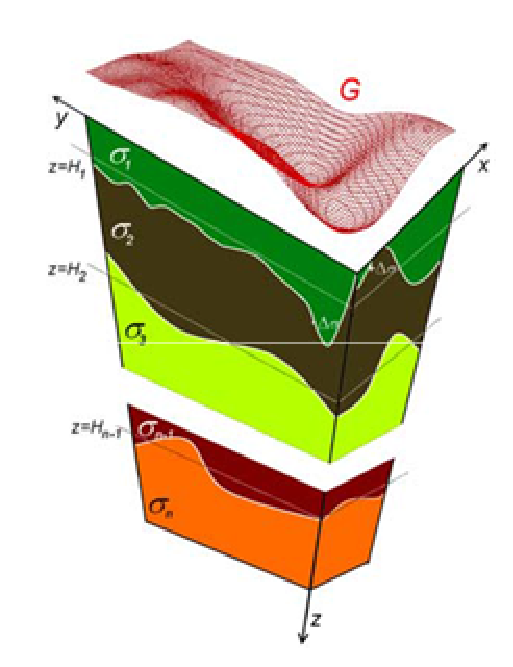
\includegraphics[height=6.0cm]{MultilayerModel}
%	\caption{Модель многослойной среды.}
%	\label{fig:multlayer}
%\end{figure}
%Пусть поверхности раздела задаются уравнениями $u_l(x,y)$, скачки плотности на них равны $\Delta\sigma_l$. поверхности имеют горизонтальные асимптотические плоскости $u_l=H_l$, т.е. $$\lim_{|x|,|y|\to\infty}|u_l(x,y)-H_l|=0.$$ Функции $u_l(x,y)$, $u=(u_1(x,y), .., u_L(x,y))$, описывающие искомые поверхности раздела сред, удовлетворяют операторному уравнению
%\begin{equation}\label{equ_grav}
%\begin{aligned}
%A(u)=\sum_{l=1}^{L}f\Delta\sigma_l\frac{1}{4\pi}\iint_D\bigg\{\frac{1}{[(x-x')^2+(y-y')^2+u_l^2(x,y)]^{1/2}} \\
%-\frac{1}{[(x-x')^2+(y-y')^2+H_l^2]^{1/2}}\bigg\}=\Delta g(x',y'),
%\end{aligned}
%\end{equation}
%где $f$~---~гравитационная постоянная, $\Delta\sigma_l(l=1,..,L)$ скачки плотности, $\Delta g(x',y')=\sum_{l=1}^{L}g_l$~--- суммарное аномальное гравитационное поле. 
%
%Предварительная обработка гравитационных данных с выделением аномального поля из измеренных гравитационных данных выполняется по методике  \cite{MarPrut2003}. Задача является недоопределенной, так как мы ищем несколько функций $u_l(x,y)$ по заданной функции $\Delta g(x',y')$. Поэтому необходимо использовать весовые множители, которые могут быть найдены по формулам из \cite{AkMarMis2013}:
%$$F=[F_1, F_2, ..., F_L]=(f_1, f_2, ..., f_{M\times L}, ..., f_{L\times M\times N})$$
%$$\to (w_1, w_2, ..., w_{L\times M\times N}),$$
%\begin{equation}\label{weght_fact_formula}
%w_i=\frac{|f_i|^\beta}{\max\limits_{i} |f_i|^\beta}, \quad \beta>1,
%\end{equation}
%где $F_l (l=1, 2, ..., L)$ --- аномальные гравитационные поля, создаваемые гравитирующими массами, находящимися на соответствующих глубинах $H_l$ и разделенных границами раздела $S_l(l=1, 2, ..., L)$.
%
%После дискретизации уравнения $(\ref{equ_grav})$ на сетке $n=M\times N$ с заданной правой частью $\Delta g(x',y')$ и аппроксимации интегрального оператора $A(u)$ по квадратурным формулам, получаем вектор правой части $F(x',y')$ размера  $M\times N$, вектор решения $u(x,y)=[u_1(x,y),..,u_L(x,y)]$ размерности $L\times M\times N$, полученный конкатенацией векторов решений, соответствующих $l$-й границе раздела, матрицу производной оператора $A'(u)$ размерности $(M\times N)\times(L\times M\times N)$, полученной приписыванием справа к матрице производной $A'(u^l)$ в точке $u^l$ матрицы $A'(u^{l+1})$, где
%\begin{equation}\label{op_grav_disc_form_mult}
%[A'(u_n^l)h_n]_{k,m}=\sum\limits_{i=1}^{M}\sum\limits_{j=1}^{N}
%\Delta x\Delta y\frac{u^l_{ij}h^l_{ij}}{[(x_k-x'_i)^2+(y_m-y'_j)^2+(u^l_{ij})^2]^{3/2}},
%\end{equation} и систему нелинейных уравнений  
%\begin{equation}\label{snl_equ}
%A_n[u]=F_n.
%\end{equation}
%Критерием останова итераций выбрана относительная норма невязки $\|A_n(u^k)-F_n\|/\|F_n\|$ точного и численного решений при достаточно малом $\varepsilon$.

%Уравнение магнитометрии при тех же предположениях, что и в задаче гравиметрии для двухслойной среды, имеет вид:
%\begin{equation}\label{equ_magn}\begin{aligned}
%\Delta J  \bigg\{&\iint_{D} \frac{H}{[(x-x')^2+(y-y')^2+H^2]^{3/2}}dx'dy' \\
%- &\iint_{D} \frac{u(x',y')}{[(x-x')^2+(y-y')^2+u^2(x',y')]^{3/2}}dx'dy' \bigg\}=\Delta G(x,y),
%\end{aligned} \end{equation}
%где $\Delta J$ -- усредненный скачок $z$-компоненты вектора намагниченности, $z=H$ -- асимптотическая плоскость, $u(x,y)$ -- функция, описывающая аномальное поле, $z=u(x,y)$ -- искомая функция, описывающая поверхность раздела сред с различными свойствами намагниченности (рис.~\ref{fig:twolayermag}). 
%\begin{figure}
%	\centering
%	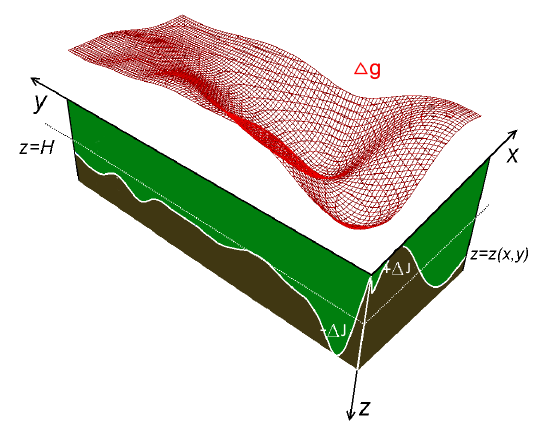
\includegraphics[height=6.0cm]{Twolaymodmag}
%	\caption{Модель двуслойной среды в задаче гравиметрии.}
%	\label{fig:twolayermag}
%\end{figure}
%Уравнение $\eqref{equ_magn}$ можно переписать в форме
%\begin{equation}\label{equ_magn_op}
%[D(u)](x,y)= \iint_{D} \frac{u(x',y')}{[(x-x')^2+(y-y')^2+u^2(x',y')]^{3/2}}dx'dy'=F(x,y),
%\end{equation}
%где $F(x,y)=D(H)-\Delta G(x,y)/\Delta J$, тогда производная оператора $D$ в точке $u^0(x,y)$ определится формулой
%$$ [A'(u^0)]h=\iint_{D} \frac{(x-x')^2+(y-y')^2-2(u^0(x',y'))^2}{[(x-x')^2+(y-y')^2+(u^0(x',y'))^2]^{5/2}}h(x',y')dx'dy'. $$
%
%После дискретной аппроксимации подобно задаче гравиметрии уравнения $\eqref{equ_magn_op}$, приходим к системе нелинейных уравнений
%\begin{equation}\label{equ_snle_mag}
%D_n(u_n)=F_n
%\end{equation}
%относительно вектора $u_n \quad (n=N\times M)$ с компонентами $u_{ij}\quad (i=1,2,...,N, j=1,2,...,M)$, при этом компоненты производной оператора $D_n$ в точке $u_{n}^{0}$ вычисляются по формуле
%\begin{equation}\label{deriv_op_mag}
%	[D'_n(u_{n}^{0})h_n]_{k,l}=\sum\limits_{i=1}^{N}\sum\limits_{j=1}^{M}
%	\Delta x\Delta y\frac{(x_k-x'_j)^2+(y_l-y'_i)^2-2(u_{ji}^0)^2}{[(x_k-x'_j)^2+(y_l-y'_i)^2+(u_{ji}^0)^2]^{5/2}}h_{ji}, 
%\end{equation}
%причем при $u_{n}^{0}=\{u^0(x'_j, y'_i), 1\le j\le M, 1\le i\le N\}=const$, $D'_n(u_n^0)$ -- симметричная матрица.

\section{Вычислительная оптимизация метода Ньютона}

Для задач (\ref{equ_snle}), (\ref{equ_snle_mag}) можно отметить, что элементы матриц $A'(u^0)$ (\ref{op_grav_disc_form}), (\ref{deriv_op_mag}) принимают наибольшие значения при малых значениях $(x-x')$ и $(y-y')$ (Рис. \ref{fig:matrixscheme}).
\begin{figure}
	\centering
	\includegraphics[height=6.0cm]{Matrix}
	\caption{Схема матрицы производной оператора $A$ в задачах грави- магнитометрии в двухслойной среде}
	\label{fig:matrixscheme}
\end{figure}
Однако при возрастании глубины $H$ асимптотической плоскости по сравнению с площадью $D$ --- размером сетки, выраженная <<ленточность>> матрицы производной оператора теряется.

Поэтому в структурных обратных задачах грави- магнитометрии при небольших относительно размера сетки глубинах $H$ при решении итерационными методами без существенной потери точности можно не учитывать значения элементов, отстоящих от диагонали далее, чем на  $\beta$-ю часть  размерности матрицы производной, то есть те значения $a_{ij}$, для которых  $j \in \{i-h(\beta),..i+h(\beta)\} $, где $h(\beta)$ --- полуширина ленты матрицы, $i, j$ --- индекс элемента. Данный подход позволяет существенно уменьшить количество вычислительных операций, перейдя от плотно заполненных матриц к матрицам ленточного вида.

В данной работе приведены результаты расчетов модельных задач гравиметрии и магнитометрии в двухслойной среде методами Ньютона и модифицированным его вариантом.

\section{Покомпонентный метод типа Ньютона}

Запишем исходное операторное уравнение (1.1) в виде:
$$P(u)=A(u)-f,$$
где $A(u)=\int_{a}^{b}\int_{c}^{d}K(x,y, x',y',u^k(x,y))dxdy$ --- интегральный оператор задачи гравиметрии (\ref{equ_grav2l}).

Итерации в методе Ньютона строятся по схеме
$$A'(u^k)(\Delta u^k)=-(A(u^k)-f),$$ где $\Delta u^k=u^{k+1}-u^k$.
То есть, для задачи гравиметрии
$$f\Delta\sigma\int_{a}^{b}\int_{c}^{d}K'_u(x,y, x',y',u^k(x,y))\Delta u^k dxdy=[A(u^k)](x',y')-f(x',y').\eqno(4.3)$$
В задаче гравиметиии на изменение гравитационного поля в правой части (4.3) наибольшее значение оказывает отклонение искомой функции точного решения $z$ от асимптотической плоскости в точке $(x',y')$. Тогда можем записать
\begin{equation}\label{comp_newt_meth_step1}
f\Delta\sigma(\Delta u^k)\int_{a}^{b}\int_{c}^{d}K'_u(x,y, x',y',u^k(x,y)) dxdy=A(u(x',y'))-f(x',y').
\end{equation}
Таким образом, величина поправки $\Delta u^k$ может быть получена как
$$\Delta u^k=\bigg[[A(u)](x',y')-f(x',y')\bigg]\bigg/f\Delta\sigma\int_{a}^{b}\int_{c}^{d}K'_u(x,y, x',y',u^k(x,y)) dxdy,$$ 
итерации осуществляются по схеме:
\begin{equation}\label{comp_newt_meth}
u^{k+1}(x',y')=u^k(x',y')-\frac{1}{\psi^k(x',y')}([A(u^k)](x',y')-f(x',y')),$$
где $$\psi^k(x',y')=f\Delta\sigma\int_{a}^{b}\int_{c}^{d}K'_u(x,y, x',y',u^k(x,y)) dxdy.
\end{equation}
В дискретной записи итерационный процесс запишется
$$u_{k,m}^{k+1}=u_{k,m}^k-\frac{1}{\psi_{k,m}^k}([A_n(u^k)]_{k,m}-f_{k,m}),\quad 1\le k \le M, \quad 1\le m \le N,$$
где $$\psi_{k,m}^k=f\Delta\sigma\sum\limits_{i=1}^{M}\sum\limits_{j=1}^{N}
\Delta x\Delta y\frac{u_{ij}}{[(x_k-x'_j)^2+(y_l-y'_i)^2+(u_{ij})^2]^{3/2}}.$$
Эту сумму $\psi_{k,m}^k$ можно интерпретировать как сумму элементов $(k\times M + l)$-й строки матрицы производной $A'_n(u_n^k)$.

Предложенный метод позволяет существенно упростить вычисления по сравнению с методом Ньютона. Вместо вычисления обратной матрицы в методе Ньютона можно вычислить вектор, состоящий из сумм элементов строк матрицы и использовать его компоненты для восстановления соответствующей компоненты вектора решения $u_n^k$. Вычислительная сложность метода Ньютона составляет $O(n^2)$, если для обращения матрицы производной $A'_n(u_n)$ использовать методы градиентного типа, в то время как вычислительная сложность покомпонентного метода $O(n)$.

\section{Покомпонентный метод типа Левенберга---Марквардта для решения обратной задачи гравиметрии для модели многослойной среды}

Рассмотрим уравнение гравиметрии для модели многослойной среды. 

Предполагается, что нижнее полупространство состоит из нескольких слоев постоянной плотности $\Delta\sigma_l(l=1,..,L)$, разделенных искомыми поверхностями $S_l$, где $L$~--- число границ раздела (рис.~\ref{fig:multlayer}). Гравитационный эффект от такого полупространства равен сумме гравитационных эффектов от всех поверхностей раздела.
\begin{figure}
	\centering
	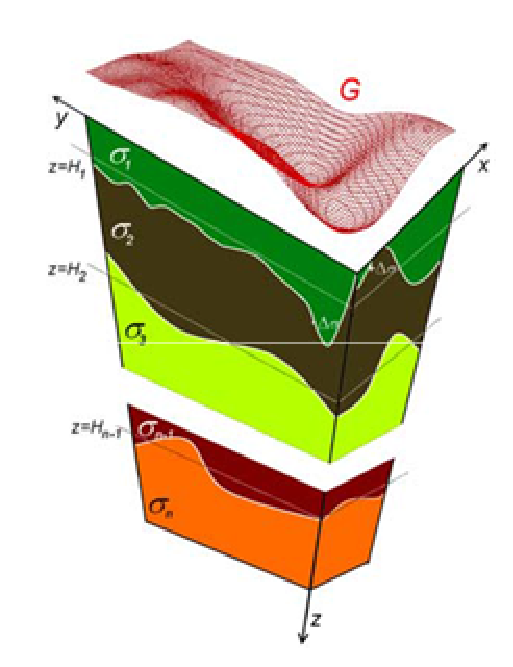
\includegraphics[height=6.0cm]{MultilayerModel}
	\caption{Модель многослойной среды.}
	\label{fig:multlayer}
\end{figure}
Пусть поверхности раздела задаются уравнениями $u_l(x,y)$, скачки плотности на них равны $\Delta\sigma_l$. поверхности имеют горизонтальные асимптотические плоскости $u_l=H_l$, т.е. $$\lim_{|x|,|y|\to\infty}|u_l(x,y)-H_l|=0.$$ Функции $u_l(x,y)$, $u=(u_1(x,y), .., u_L(x,y))$, описывающие искомые поверхности раздела сред, удовлетворяют операторному уравнению
\begin{equation}\label{equ_grav}
\begin{aligned}
A(u)=\sum_{l=1}^{L}f\Delta\sigma_l\frac{1}{4\pi}\iint_D\bigg\{\frac{1}{[(x-x')^2+(y-y')^2+u_l^2(x,y)]^{1/2}} \\
-\frac{1}{[(x-x')^2+(y-y')^2+H_l^2]^{1/2}}\bigg\}=\Delta g(x',y'),
\end{aligned}
\end{equation}
где $f$~---~гравитационная постоянная, $\Delta\sigma_l(l=1,..,L)$ скачки плотности, $\Delta g(x',y')=\sum_{l=1}^{L}g_l$~--- суммарное аномальное гравитационное поле. 

Предварительная обработка гравитационных данных с выделением аномального поля из измеренных гравитационных данных выполняется по методике  \cite{MarPrut2003}. Задача является недоопределенной, так как мы ищем несколько функций $u_l(x,y)$ по заданной функции $\Delta g(x',y')$. Поэтому необходимо использовать весовые множители, которые могут быть найдены по формулам из \cite{AkMarMis2013}:
$$F=[F_1, F_2, ..., F_L]=(f_1, f_2, ..., f_{M\times L}, ..., f_{L\times M\times N})$$
$$\to (w_1, w_2, ..., w_{L\times M\times N}),$$
\begin{equation}\label{weght_fact_formula}
w_i=\frac{|f_i|^\beta}{\max\limits_{i} |f_i|^\beta}, \quad \beta>1,
\end{equation}
где $F_l (l=1, 2, ..., L)$ --- аномальные гравитационные поля, создаваемые гравитирующими массами, находящимися на соответствующих глубинах $H_l$ и разделенных границами раздела $S_l(l=1, 2, ..., L)$.

После дискретизации уравнения $(\ref{equ_grav})$ на сетке $n=M\times N$ с заданной правой частью $\Delta g(x',y')$ и аппроксимации интегрального оператора $A(u)$ по квадратурным формулам, получаем вектор правой части $F(x',y')$ размера  $M\times N$, вектор решения $u(x,y)=[u_1(x,y),..,u_L(x,y)]$ размерности $L\times M\times N$, полученный конкатенацией векторов решений, соответствующих $l$-й границе раздела, матрицу производной оператора $A'(u)$ размерности $(M\times N)\times(L\times M\times N)$, полученной приписыванием справа к матрице производной $A'(u^l)$ в точке $u^l$ матрицы $A'(u^{l+1})$, где
\begin{equation}\label{op_grav_disc_form_mult}
[A'(u_n^l)h_n]_{k,m}=\sum\limits_{i=1}^{M}\sum\limits_{j=1}^{N}
\Delta x\Delta y\frac{u^l_{ij}h^l_{ij}}{[(x_k-x'_i)^2+(y_m-y'_j)^2+(u^l_{ij})^2]^{3/2}},
\end{equation} и систему нелинейных уравнений  
\begin{equation}\label{snl_equ}
A_n[u]=F_n.
\end{equation}

Для решения задач (\ref{equ_grav2l}), (\ref{equ_grav}) предлагается метод покомпонентного типа, основанный на идее метода Левенберга---Марквардта. 

Для аппроксимации решения уравнения (\ref{equ_2lop}) метод Левенберга---Марквардта (МЛМ) имеет вид:
\begin{equation}
u^{k+1}=u^k-\gamma[A'(u^k)^*A'(u^k)+\alpha I]^{-1} A'(u^k)^*(A(u^k)-f_\delta),
\end{equation}
где $A'(u^k)^*$ --- оператор, сопряженный к производной оператора $A$ задачи $A'(u)$, $\alpha>0$~--~параметр регуляризации, $\|f-f_\delta\|\le \delta.$
 
В работах В.В. Васина \cite{Vasin_2012}, \cite{VasPer_2011} был исследован метод Левенберга---Марквардта
\begin{equation}\label{LM_Vasin}
u^{k+1}=u^k-\gamma[A'(u^k)^*A'(u^k)+\bar{\alpha} I]^{-1} [A'(u^k)^*(A(u^k)-f_\delta)+\alpha (u-u^0)]
\end{equation} и его модифицированный вариант
\begin{equation}\label{LM_modif_Vasin}
u^{k+1}=u^k-\gamma[A'(u^0)^*A'(u^0)+\bar{\alpha} I]^{-1} [A'(u^k)^*(A(u^k)-f_\delta)+\alpha (u-u^0)]
\end{equation} для решения регуляризованного уравнения
$$A'(u)^*(A(u)-f_\delta)+	\alpha (u-u^0)=0,$$
где $\gamma$ --- демпфирующий множитель, $u^0$ --- некоторое приближение к $u_\alpha$, $\alpha>0$. На основании выводов, сделанных М.Ю. Кокуриным \cite{Kok_2010} о свойствах градиента $\Phi_\alpha '(u)$ тихоновского функционала $$\Phi_\alpha(u)=(1/2)(\|A(u)-f_\delta\|^2+\alpha\|u-\xi\|^2)$$ было установлено, что при выборе параметров $\bar{\alpha}$, $\alpha$, $\gamma$ имеет место сильная сходимость итераций (\ref{LM_Vasin}), (\ref{LM_modif_Vasin}) к регуляризованному решению $u_\alpha$.

По аналогии с покомпонентным методом типа Ньютона (\ref{comp_newt_meth}), можно выполнить прием вынесения значимой компоненты за знак интегрального оператора, как в (\ref{comp_newt_meth_step1}) и запишем итерационную последовательность восстановления каждой из неизвестных границ $u_l$
\begin{equation}\label{comp_lm_meth}
u_l^{k+1}=u_l^k-\gamma\frac{1}{\varphi_l}\Lambda[ A'(u_l^k)^T(A(u^k)-f_\delta)+\alpha (u_l^k-u_l^0)],
\end{equation}
где $l$ -- номер границы раздела, $l=1,..,L$, $\Lambda$ --- диагональная матрица, состоящая из весовых множителей, 
\begin{equation*}
\begin{aligned}
\varphi_l=\bigg[ f\Delta\sigma\int_{a}^{b}\int_{c}^{d}
K'_u(x',y', x, y, u_l^k(x,y))dx'dy'\bigg] \notag \\ \times\bigg[f\Delta\sigma\int_{a}^{b}\int_{c}^{d}K'_u(x,y, x',y',u_l^k(x,y))dxdy\bigg], 
\end{aligned}
\end{equation*} 
где $K'_u(x',y', x, y, u_l^k(x,y))$ --- функция ядра, транспонированного к ядру $K'_u(x,y,$ $ x',y',u^k(x,y))$. Величина $\varphi_l$ зависит от $u_l^k$.
Итерационный процесс (\ref{comp_lm_meth}) перепишем в дискретной форме
\begin{equation}\label{comp_lm_meth_disc}
u_{l,i}^{k+1}=u_{l,i}^k-\gamma\frac{1}{\varphi_{l,i}}w_{l,i}\bigg[ \{A'(u_l^k)^T(A(u^k)-f_\delta)\}_i+\alpha (u_{l,i}^k-u_{l,i}^0)\bigg],
\end{equation}
где $w_{l,i}$ --- $i$-й весовой множитель, зависящий от $l$-й границы раздела,
\begin{equation*}
\begin{aligned}
\varphi_{l,i}=\bigg[ f\Delta\sigma\sum\limits_{k=1}^{N}
\sum\limits_{m=1}^{M}
K'_u(x'_k,y'_m, \{x, y\}_i, u_{l,i}^k) \Delta x' \Delta y'\bigg] \notag \\ \times\bigg[f\Delta\sigma\sum\limits_{k=1}^{N}
\sum\limits_{m=1}^{M}K'_u(x_k,y_m, \{x',y'\}_i,u_l^k(x_k,y_m))\Delta x \Delta y\bigg]. 
\end{aligned}
\end{equation*}

Преимущества покомпонентного метода типа Левенберга---Марквардта в низкой вычислительной сложности. Здесь не требуется вычисления матрицы $A'(u^k)^T A'(u^k)+\alpha I$. Это делает метод более экономичным в численных расчетах по сравнению с (\ref{LM_Vasin}), (\ref{LM_modif_Vasin}), где вычислительная сложность алгоритмов достигает $O(n^3)$ в силу умножения матриц $A'(u^k)^T A'(u^k)$ и обращения матрицы $A'(u^k)^T A'(u^k)+\alpha I$. Вычислительная сложность (\ref{comp_lm_meth}) составляет $O(n^2)$ потому что самыми затратными по времени операциями являются вычисление элементов матрицы $A'(u^k)^T$ и матрично-векторные умножения.

\newpage
\section{Численные эксперименты}

{\bfseries 3.4.1.} Рассматривается эксперимент по восстановлению границы раздела в двухслойной среде модифицированным методом Ньютона и его оптимизированным вариантом (c использованием ленточной матрицы производной оператора) с распараллеливанием вычислений. Решается модельная задача.

Точное решение уравнения гравиметрии, определяющее поверхность раздела сред, задается формулой
$$\hat{u}(x,y)=5-3.21e^{-(x/10.13-6.62)^6-(y/9.59-2.93)^6}-2.78e^{-(x/9.89-4.12)^6-(y/8.63-7.435)^6}$$ 
\begin{equation}\label{exact_exp3.4.1}
+3.19e^{-(x/9.89-4.82)^6-(y/8.72-4.335)^6},
\end{equation}
\begin{figure}
	\centering
	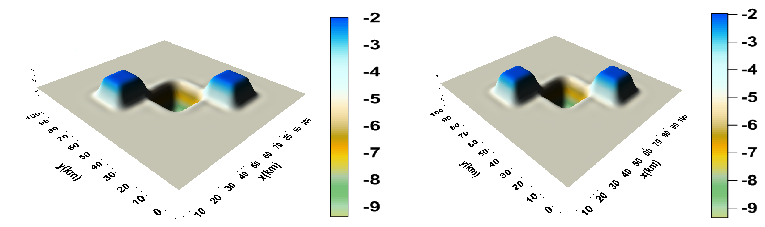
\includegraphics[width=\textwidth]{gravy_kiev2014}
	\caption{Модельная поверхность (слева) и приближенное решение (справа) задачи гравиметрии.}
	\label{fig:gravy_kiev2014}
\end{figure}
Поверхность задана на области $D=\{0\le x\le 270, 0\le y\le 300\}$, с асимптотической плоскостью $H=5$, размерами шагов сетки $\Delta x=\Delta y=0.3$, скачком плотности $\Delta\sigma=0.2$ г/см$^3$.

Точное решение уравнения магнитометрии, определяющее поверхность раздела сред, задается формулой
$$\hat{u}(x,y)=5-2e^{-(x/10-3.5)^6-(y/10-2.5)^6}-3e^{-(x/10-5.5)^6-(y/10-4.5)^6},$$
\begin{figure}
	\centering
	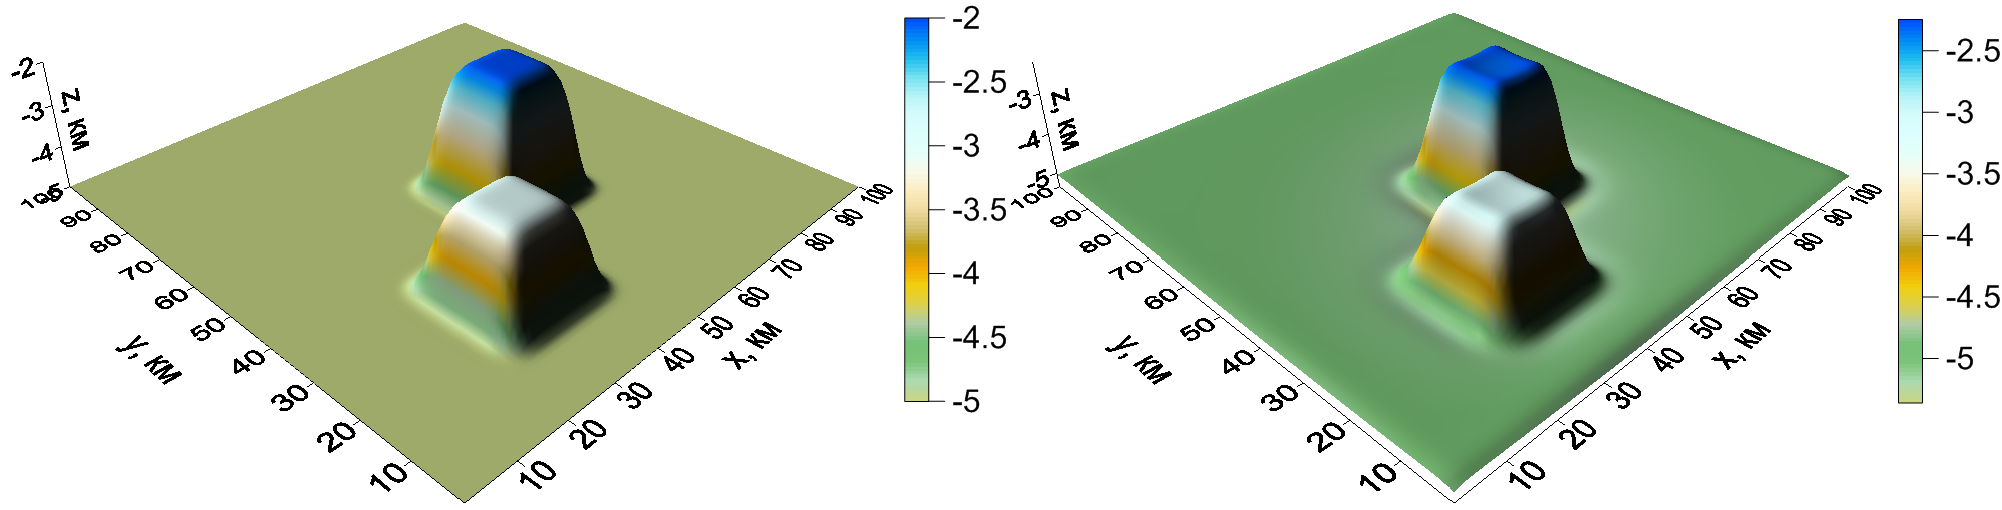
\includegraphics[width=\textwidth]{magne_kiev2014}
	\caption{Модельная поверхность (слева) и приближенное решение (справа) задачи магнитометрии.}
	\label{fig:magne_kiev2014}
\end{figure}
Поверхность задана на области $D=\{0\le x\le 300, 0\le y\le 300\}$, $H=5$, $\Delta x=\Delta y=0.3$, скачком вектора намагниченности $\Delta J=0.4$ А/м. В таблицах \ref{table3.1}, \ref{table3.2} приведены результаты расчетов, критерий останова итераций 
$\delta=\|u_e-u_a\|/\|u_e\|\le 0.025$, параметры регуляризации $\alpha=\bar{\alpha}=10^{-3}$, полуширина ленты матрицы производной $\beta=1/4$ для задачи гравиметрии и $\beta=1/5$ для задачи магнитометрии. Обозначение $\Delta=\|A(u^k)+\alpha(u^k-u^0)-f_\delta\|/\|f_\delta\|$ --- относительная норма регуляризованной невязки, $N$ --- число итераций, $T_1$ --- время счета последовательной программы, $T_8$ --- время счета программы на многоядерном процессоре intel Xeon с использованием 8 ядер процессора.
\begin{table}[]
	\centering
	\caption{Решение обратной задачи гравиметрии в двухслойной среде}
	\label{table3.1}
	\begin{tabular}{|p{0.3\textwidth}|p{0.05\textwidth}|l|l|l|}
		\hline
		\multicolumn{1}{|c|}{Метод}        & \multicolumn{1}{c|}{$N$} &
		\multicolumn{1}{c|}{$\Delta$} & \multicolumn{1}{c|}{$T_1$} & \multicolumn{1}{c|}{$T_8$} \\ \hline
		Метод Ньютона                      &  3        & 0.041                          &       22 мин                  &     2 мин 40 сек                 \\ \hline
		Модифицированный метод Ньютона     &         5           & 0.042            & 32 мин                  & 4 мин                   \\ \hline
		Метод Ньютона с ленточной матрицей &  4               & 0.041                    & 24 мин                  & 3 мин                   \\ \hline
	\end{tabular}
\end{table}
\begin{table}[]
	\centering
	\caption{Решение обратной задачи магнитометрии в двухслойной среде}
	\label{table3.2}
	\begin{tabular}{|p{0.25\textwidth}|p{0.05\textwidth}|l|l|l|}
		\hline
		\multicolumn{1}{|c|}{Метод}        & \multicolumn{1}{c|}{$N$} &
		\multicolumn{1}{c|}{$\Delta$} &
		\multicolumn{1}{c|}{$T_1$} & \multicolumn{1}{c|}{$T_8$} \\ \hline
		Метод Ньютона                      &   3             & 0.05                  &     9 мин                   &      1 мин 30 сек                 \\ \hline
		Модифицированный метод Ньютона     &              6           & 0.051           & 15 мин 30 сек                & 2 мин                   \\ \hline
		Метод Ньютона с ленточной матрицей &   5                    & 0.05               & 9 мин 36 сек                & 1 мин 12 сек                 \\ \hline
	\end{tabular}
\end{table}

Также были проведены эксперименты в случае с возмущенной правой частью. На $f$ был наложен гауссовский шум с математическим ожиданием $\mu_g=0.5$ и дисперсией $\sigma_g=0.7$ в случае гравитационного поля и $\mu_m=0.002$ и дисперсией $\sigma_m=0.001$ для магнитного поля. В первом случае шум составляет 16\%, во втором --- 6\%. На рис.\ref{fig:exp341_mmn_gravy}, \ref{fig:exp341_mmn_magne} изображены возмущенные поля и восстановленные модифицированным методом Ньютона поверхности раздела сред.
\begin{figure}
	\centering
	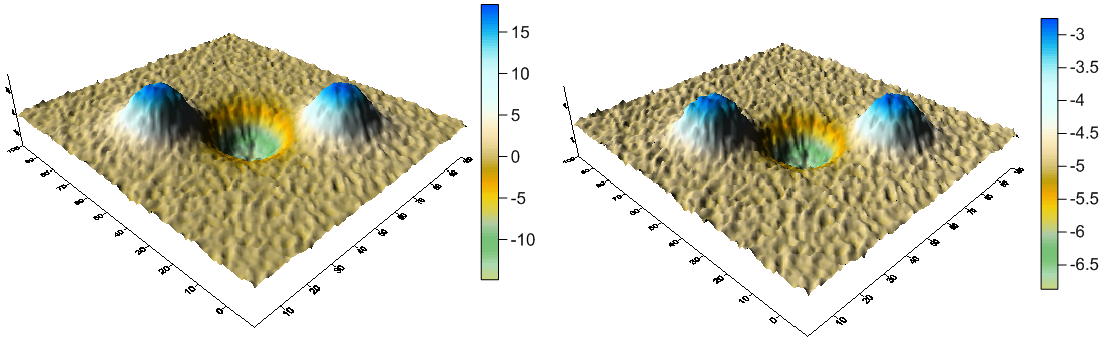
\includegraphics[width=\textwidth]{exp341_mmn_gravy}
	\caption{Гравитационное поле (слева) и приближенное решение (справа) ММН.}
	\label{fig:exp341_mmn_gravy}
\end{figure}
\begin{figure}
	\centering
	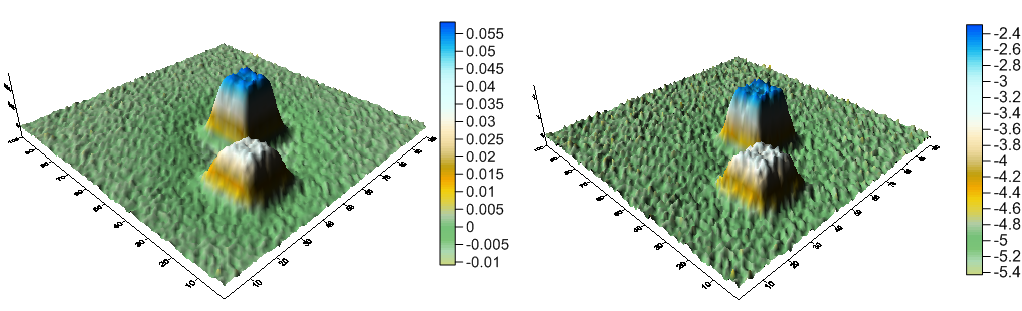
\includegraphics[width=\textwidth]{exp341_mmn_magne}
	\caption{Магнитное поле (слева) и приближенное решение (справа) ММН.}
	\label{fig:exp341_mmn_magne}
\end{figure}

В таблицах \ref{table3.3}, \ref{table3.4} приведены результаты расчетов, где $\gamma$ --- параметр регулировки шага. Критерий останова --- относительная погрешность $\delta<10^{-1}$. Можно сделать вывод, что исключение из матрицы производной оператора $A'(u^k)$ элементов, далеко отстоящих от диагонали, почти не влияет на сходимость метода Ньютона. Данные, полученные в ходе расчетов, не проиворечат теоремам главы 2 о сходимости методов Ньютона и его модифицированного варианта. В частности, в задаче гравиметрии для методов понадобилось уменьшать параметр $\gamma$ для обеспечения сходимости итерационных процессов. Замена матрицы производной на ленточную не оказывает существенного влияния на скорость сходимости за счет почти не измененного параметра $N_1$ в оценках теоремы \ref{teo4.1}. Оба алгоритма обладают высокой степенью параллелизма, что дает $n$-кратное уменьшение времени счета программ при использовании $n$ ядер процессора.
\begin{table}[]
	\centering
	\caption{Результаты для задачи гравитометрии с шумом}
	\label{table3.3}
	\begin{tabular}{|l|l|p{0.05\textwidth}|c|}
		\hline
		\multicolumn{1}{|c|}{Метод}                                                   & \multicolumn{1}{c|}{Параметры}              & \begin{tabular}[c]{@{}l@{}} $N$ \end{tabular} & $\Delta$ \\ \hline
		Метод Ньютона                                                                 & $\gamma = 0.2$, $\alpha=0.1$, $\bar\alpha=1$   & 5                   & 0.47     \\ \hline
		\begin{tabular}[c]{@{}l@{}}Модифицированный \\ метод Ньютона\end{tabular}     & $\gamma =0.2$, $\alpha=0.1$, $\bar\alpha=1$ & 5                   & 0.46     \\ \hline
		\begin{tabular}[c]{@{}l@{}}Метод Ньютона \\ с ленточной матрицей\end{tabular} & $\gamma =0.2$, $\alpha=0.1$, $\bar\alpha=1$ & 5                   & 0.46     \\ \hline
	\end{tabular}
\end{table}

\begin{table}[]
	\centering
	\caption{Результаты для задачи магнитометрии с шумом}
	\label{table3.4}
	\begin{tabular}{|l|l|p{0.05\textwidth}|c|}
		\hline
		\multicolumn{1}{|c|}{Метод}        & \multicolumn{1}{c|}{Параметры}              & \begin{tabular}[c]{@{}l@{}} $N$ \end{tabular} & $\Delta$ \\ \hline
		Метод Ньютона                      & $\gamma =1$, $\alpha=10^{-3}$, $\bar\alpha=0.1$   & 5                   & 0.49     \\ \hline
		\begin{tabular}[c]{@{}l@{}}Модифицированный \\ метод Ньютона\end{tabular}   & $\gamma = 1$, $\alpha=10^{-3}$, $\bar\alpha=0.1$ & 6                   & 0.49     \\ \hline
		\begin{tabular}[c]{@{}l@{}}Метод Ньютона \\ с ленточной матрицей\end{tabular} & $\gamma = 1$, $\alpha=10^{-3}$, $\bar\alpha=0.1$ & 5                   & 0.49     \\ \hline
	\end{tabular}
\end{table}

{\bfseries 3.4.2.} Рассматривается эксперимент по восстановлению границы раздела в двухслойной среде модифицированным методом Ньютона (ММН) и покомпонентным методом типа Ньютона (ПМН) с распараллеливанием вычислений на многоядерном процессоре. Решается модельная задача. Точное решение уравнения гравиметрии, определяющее поверхность раздела сред, задается формулой (\ref{exact_exp3.4.1}) на области $D=\{0\le x\le 300, 0\le y\le 330\}$, с асимптотической плоскостью $  H=5$, размерами шагов сетки $\Delta x=\Delta y=0.33$, скачком плотности $\Delta\sigma=0.21$ г/см$^3$.
\begin{figure}
	\centering
	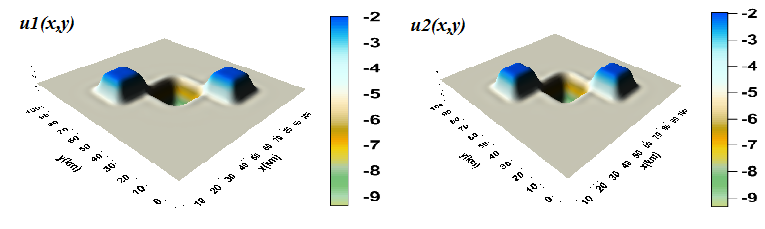
\includegraphics[width=\textwidth]{gravy_kiev2015_methods}
	\caption{Решение, полученное ММН (слева) и решение, полученное ПМН (справа).}
	\label{fig:gravy_kiev2015_methods}
\end{figure}
На рис. \ref{fig:gravy_kiev2015_methods} изображены восстановленные поверхности обоими методами. Вычисления производились для сеток размерами $100\times 110$, $300\times 330$. Параметры регуляризации $\alpha=\bar{\alpha}=10^{-3}$, демпфирующий параметр $\gamma=1.8$ для покомпонентного метода Ньютона. Критерий останова итераций $\delta=\|u_e-u_a\|/\|u_e\|<10^{-2},$ $N$ --- число итераций, 
$\Delta=\|A(u^k)+\alpha(u^k-u^0)-f_\delta\|/\|f_\delta\|$ --- относительная норма регуляризованной невязки, $T_1$ --- время счета последовательной программы, $T_8$ --- время счета программы на многоядерном процессоре intel Xeon с использованием 8 ядер процессора.
\begin{table}[]
	\centering
	\caption{Сравнение ММН и ПМН}
	\label{table3.5}
	\begin{tabular}{|p{0.15\textwidth}|p{0.05\textwidth}|c|c|c|c|}
		\hline
		\multicolumn{1}{|c|}{\textbf{Метод}} & \textbf{$N$} &
		\textbf{$\Delta$} & \textbf{$T_1$ (100$\times$110)} & \textbf{$T_1$ (300$\times$330)} & \textbf{$T_8$ (300$\times$330)} \\ \hline
		ММН       & 16             &    0.002     & 21 сек          & 25 мин          & 3 мин 25 сек    \\ \hline
		ПМН    & 21             &     0.002    & 13 сек          & 11 мин          & 1 мин 38 сек    \\ \hline
	\end{tabular}
\end{table}

Также были проведены вычисления для возмущенной правой части из эксперимента 3.4.1. На рис. \ref{fig:exp342_mmn_cmn_noise} изображены восстановленные поверхности обоими методами из возмущенной правой части. Результаты приводятся в таблице \ref{table3.6}. Критерием останова послужило условие $\Delta=\|A(u^k)+\alpha(u^k-u^0)-f_\delta\|/\|f_\delta\|<0.18$, $\delta=\|u_e-u_a\|/\|u_e\|<10^{-2}$.
\begin{figure}
	\centering
	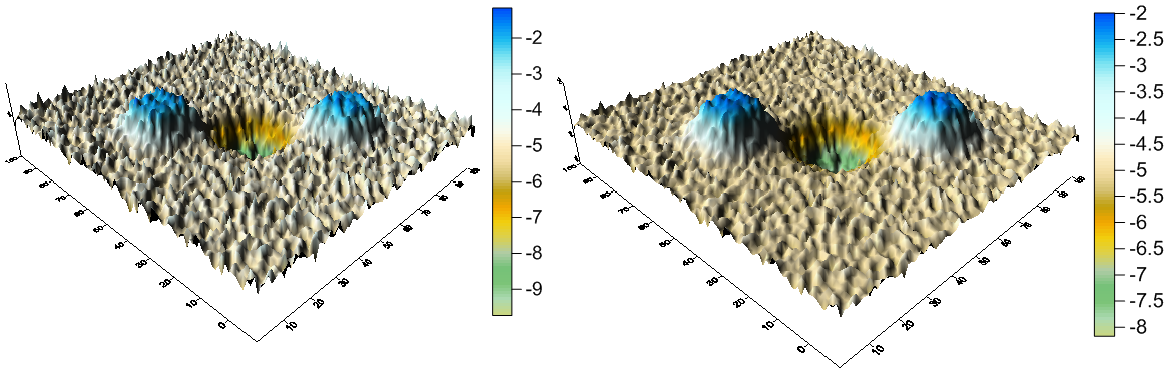
\includegraphics[width=\textwidth]{exp342_mmn_cmn_noise}
	\caption{Решение, полученное ММН (слева) и решение, полученное ПМН (справа).}
	\label{fig:exp342_mmn_cmn_noise}
\end{figure}
\begin{table}[]
	\centering
	\caption{Сравнение ММН и ПМН для задачи с шумом}
	\label{table3.6}
	\begin{tabular}{|l|l|c|c|}
		\hline
		\multicolumn{1}{|c|}{Метод} & \multicolumn{1}{c|}{Параметры}              & $N$ & $\delta$ \\ \hline
		ММН                         & $\gamma =0.4$, $\alpha=0.1$, $\bar\alpha=10$ & 38   & 0.22     \\ \hline
		ПМН                         & $\gamma =1$, $\alpha=1$, $\bar\alpha=10$    & 7   & 0.078    \\ \hline
	\end{tabular}
\end{table}

Размерность матрицы производной в модифицированном методе Ньютона $A'(u^0)$ при сетке $300\times330$ составляет $9.9 * 10^4\times 9.9 * 10^4$, что сильно увеличило время счета задачи методом ММН, в отличие от предыдущего эксперимента 3.4.1. Проведенные эксперименты наглядно демонстрируют выгоду использования ПМН для решения обратных задач на больших сетках. На улучшение результата по сглаживанию шума оказал влияние подбор регуляризующих параметров $\bar{\alpha}, \alpha$. Также решение, полученное ПМН оказалось более <<сглаженным>>, чем ММН, что говорит о большей устойчивости к шуму.
 
 {\bfseries 3.4.3.} Рассматривается эксперимент по восстановлению границы раздела в двухслойной среде покомпонентным методом типа Ньютона и покомпонентным методом типа Левенберга--Марквардта (ПЛМ)  с распараллеливанием вычислений на многоядерном процессоре.
 
 Точное решение уравнения гравиметрии, определяющее поверхность раздела сред, задается формулой
 $$\hat{u}(x,y)=5+4e^{-(x/10-3.5)^4-(y/10-2.5)^4}-3e^{-(x/10-5.5)^4-(y/10-4.5)^4},$$
 на области $D=\{0\le x\le 512, \,\,0\le y\le 512\}$,  $H=5$, $\Delta x=\Delta y=1$, $\Delta\sigma=0.2$ г/см$^3$.
 \begin{figure}
 	\centering
 	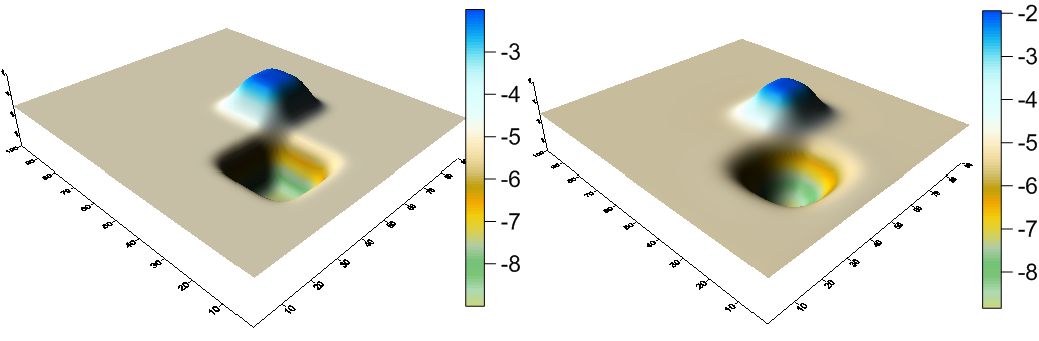
\includegraphics[width=\textwidth]{gravy_nov2014}
 	\caption{Точное решение (слева) приближенное решение ПЛМ (справа).}
 	\label{fig:gravy_nov2014}
 \end{figure}
 На рис. \ref{fig:gravy_nov2014} изображены восстановленные поверхности обоими методами. Вычисления производились для сетки размерами $512\times 512$. Параметры регуляризации $\alpha=\bar{\alpha}=10^{-3}$, демпфирующий параметр $\gamma=1.6$ для покомпонентного метода Ньютона. Критерий останова итераций $\delta=\|u_e-u_a\|/\|u_e\|<0.025,$ $N$ --- число итераций, 
 $\Delta=\|A(u^k)+\alpha(u^k-u^0)-f_\delta\|/\|f_\delta\|$ --- относительная норма регуляризованной невязки, $T_1$ --- время счета последовательной программы, $T_8$ --- время счета программы на многоядерном процессоре intel Xeon с использованием 8 ядер процессора.
 \begin{table}[]
 	\centering
 	\caption{Сравнение ПМН и ПМЛМ}
 	\label{table3.7}
 	\begin{tabular}{|p{0.1\textwidth}|c|c|c|c|}
 		\hline
 		\multicolumn{1}{|c|}{\textbf{Метод}}            & \textbf{$N$} & \textbf{$\Delta$} & \textbf{$T_1$ (512$\times$512)} & \textbf{$T_8$ (512$\times$512)} \\ \hline
 		ПМН               & 3         & 0.01             & 11 мин 27 сек   & 1 мин 44 сек    \\ \hline
 		ПЛМ & 3   &     0.01              & 2 ч 2 мин       & 16 мин          \\ \hline
 	\end{tabular}
 \end{table}
 
% \begin{table}[]
% 	\centering
% 	\caption{Сравнение ПМН и ПМЛМ}
% 	\label{table3.8}
% 	\begin{tabular}{|l|c|c|l|l|l|l|l|}
% 		\hline
% 		\multicolumn{1}{|c|}{\multirow{2}{*}{\textbf{Метод}}} & \multirow{2}{*}{\textbf{$N$}} & \multirow{2}{*}{\textbf{$\Delta$}} & \multicolumn{2}{c|}{\textbf{Сетка 512$\times$512}}                        & \multicolumn{3}{c|}{\textbf{Сетка 1000$\times$1000}}                                                            \\ \cline{4-8} 
% 		\multicolumn{1}{|c|}{}                                &                               &                                    & \multicolumn{1}{c|}{\textbf{$T_1$}} & \multicolumn{1}{c|}{\textbf{$T_8$}} & \multicolumn{1}{c|}{\textbf{$T_1$}} & \multicolumn{1}{c|}{\textbf{$T_8$}} & \multicolumn{1}{c|}{\textbf{$T_n$}} \\ \hline
% 		ПМН                                                   & 3                             & 0.01                               & 11 мин. 27 сек                      & 1 мин. 44 сек                       & 16 ч.                               & 2 ч.                                & 20 мин.                             \\ \hline
% 		ПЛМ                                                   & 3                             & 0.01                               & 2 мин. 2 сек                        & 16 мин.                             & 5 дней 14 ч.                        & 17 ч.                               & 3 ч.                                \\ \hline
% 	\end{tabular}
% \end{table}

{\bfseries 3.4.4.} Рассматривается эксперимент по восстановлению границ раздела сред в многослойной среде (4 слоя с разной плотностью) в задаче гравиметрии на основе квазиреального аномального поля методами: регуляризованный Левенберга--Марквардта и покомпонентный типа Левенберга--Марквардта.
%% Глава 4
%\chapter{Комплекс программ}

В данной главе рассматриваются программные реализации алгоритмов на основе методов, описанных в первых трех главах. 

\newpage
\section{Описание комплекса программ}
\section{Рекомендации по использованию}

% Заключение
\conclusion

Приведены основные результаты диссертационной работы.

1. Для нелинейного уравнения с монотонным оператором доказаны теоремы сходимости для регуляризованного метода Гаусса -- Ньютона, построены регуляризованные методы градиентного типа, названные нелинейными аналогами $\alpha$-процессов, для нелинейного уравнения с монотонным оператором доказаны теоремы сходимости для них, доказана сильная фейеровость итерационных процессов.

2. Для задачи с немонотонным оператором, производная которого имеет неотрицательный спектр, доказаны теоремы сходимости методов Ньютона, нелинейных $\alpha$-процессов и их модифицированных вариантов.

3. Предложена вычислительная оптимизация метода Ньютона и его модифицированного варианта при решении задач с матрицей производной, близкой к ленточной; на примере решения обратной задачи гравиметрии продемонстрирована вычислительная экономичность модификации. 

Для решения систем нелинейных интегральных уравнений  с ядром оператора структурной обратной задачи гравиметрии в двуслойной среде предложен покомпонентный метод, основанный на методе Ньютона. Для решения систем нелинейных уравнений  структурных обратных задач гравиметрии в многослойной среде предложен подход на основе метода Левенберга -- Марквардта --- покомпонентный метод типа Левенберга -- Марквардта.

Программные реализации предложенных методов поддерживают использование многоядерных процессоров, для покомпонентных методов и метода Ньютона и модифицированного варианта реализованы также программы для вычислений на графических процессорах.

В дальнейшей научной работе автора предполагается исследование на сходимость покомпонентных методов типа Ньютона и Левенберга -- Марквардта.


% Словарь терминов
%% Словарь терминов
\dict

\textbf{Термин} "--- определение.


% Список литературы
% Выделять курсивом
\let\BibEmph=\emph
%\bibliographystyle{gost705s}
%\bibliographystyle{utf8gost705u}
%\bibliography{thesis}
%\printbibliography

\printbibliography[
	notkeyword=own,
	heading=bibintoc
	]
\printbibliography[
	keyword=own,
	heading=bibintoc,
	title={Публикации автора}
	]

% Список иллюстративного материала
%\listoffigures

% Приложения
%\appendix
%\chapter{Название приложения}

%\pageref{LastPage}

\end{document}
